\documentclass[10pt,a4paper,titlepage]{report}
\usepackage[utf8]{inputenc}
\usepackage[T1]{fontenc}
\usepackage{amsmath}
\usepackage{amsfonts}
\usepackage{amssymb}
\usepackage{graphicx}
\usepackage{svg}
\usepackage{subfig}
\usepackage{todonotes}
\usepackage{hyperref}
\usepackage{geometry}
\usepackage{tcolorbox}
\newtcolorbox{hindsight}{colback=red!5!white,colframe=red!75!black,fonttitle=\bfseries,title=Hindsight}


\usepackage{minted}
\usepackage{xcolor}
\definecolor{LightGray}{gray}{0.9}

\setmintedinline {
bgcolor=white,
framesep=0mm,
}


\setminted{
framesep=2mm,
baselinestretch=1.2,
bgcolor=LightGray,
fontsize=\footnotesize,
linenos
}


% How to insert code:
% \begin{minted}{c}
% // Test code
% bla
% \end{minted}

% How to inline code
% \mintinline{c}{bal} 

% TODO: Replace the title with your own
\title{Bellyflop OS Report}
\author{Group 11}


\begin{document}
	
    
	\maketitle
	\begin{figure}
	    \centering
	    
\includegraphics{figs/belly_flo_orig.png}
	    \caption{Bellyflop OS}
	    \label{fig:belly_flop}
	\end{figure}

% 	\chapter{DEMO Delete later}
	
% 	TODO: WRite your report. Please also mention whether you have any limitations
% 	(e.g., limit of mapped memory, ...) and/or whether you've done extra challenges.
% 	\\
% 	\\
% 	This could be our demo, just putting this here as shared notes.
% 	\begin{itemize}
% 	    \item Start the device and use the terminal to run the TCP/ UDP servers.
% 	    \item Demonstrate Echo servers
% 	    \item Take over shell with the remote shell login.
% 	    \item create a file and edit it.
% 	    \item load a program from disk.
% 	    \item TODO: Show stuff by using the shell over the remote login.
	    
% 	\end{itemize}
	
	\tableofcontents
	
	\chapter{Testing Framework}

Testing the code you write is probably just as important as actually writing the code.
This is especially true when you are working on a complex system with many interacting components like an Operating System.

We therefore want to start by showing the Testing Framework we created for this project.
It proved useful throughout the different chapters of the course because it greatly simplified and standardized the way we would write tests.

% We created some macro magic that lets you create and run tests by doing this:
It uses some "macro magic" to create and group different test cases together.
These groups of commands can then be executed by using the \mintinline{c}{RUN_TESTS(<group>)} command.
It shows you if the tests succeeded or failed, and, if they failed, where and why they failed.

\begin{minted}{c}
CREATE_TEST(test_name1, group_name, 
{
    errval_t err;
    err = ...
    TEST_REQUIRE_OK(err);
    err = ...;
    TEST_REQUIRE_FAIL_WITH(err, SOME_ERR);
})

CREATE_TEST(test_name2, group_name, 
{
    // This makes a test fail but doesn't abort the execution.
    TEST_CHECK(1 == 2);
    // This makes a test fail and aborts execution of this test (but not the group).
    TEST_REQUIRE(1 == 2); 
})

// ...

void run_testing(void) {
    RUN_TESTS(group_name);
}
\end{minted}
This is how it looks like when a test fails (in red):
\begin{minted}{sh}
/lib/grading/group_name_tests.h:12: 1==2 failed
/lib/grading/group_name_tests.h:13: 1==2 failed
Test test_name2 in group_name failed.
1/8 tests in group_name failed.
\end{minted}
This is how it looks like when all tests pass (in green):
\begin{minted}{sh}
All 8/8 tests in group_name succeeded.
\end{minted}
	\chapter{Memory Allocator}

As the first step, we had to implement a physical memory allocator.
This would serve as the basis for everything else. 
It thus had to be as robust as possible or it could cause major pains when discovering bugs later in the project.

We chose to implement a "Next Fit" Allocation strategy, maintaining the free memory blocks in a linked list. We picked Next Fit because it was recommended in the lecture. There was also a plan to go for a more sophisticated approach should we run into performance issues. In the end, the Memory Allocator was never a bottleneck for us.

\section{Free List}
The free list is composed of two nested lists.

The memory manager is initialized with a set of memory region capabilities.
These memory region capabilities each have their own node in a circular linked list.
We will refer to this list as the region list.

Each node in the region list also contains a second linked list that keeps track of which sections of the region are free.
We call this the sections list.
It is a sorted list of disjoint intervals of free memory.
Two nodes with bordering intervals are always merged into one node.
This makes allocation easy and quick.

The data structure also keeps track of the last position that memory was allocated from.
This is needed for the Next Fit strategy.

\begin{figure}[ht]
    \centering
    \scalebox{0.5}{\includesvg{./figs/free_list.svg} }

    \caption{General Overview of the Free List. Memory region capabilities are stored in a circular list. Each of the nodes maintains its own list to keep track of free sections in the region.}
    \label{fig:free_list}
\end{figure}

\section{Allocating memory}
The interface allows the user to specify both size and the alignment requirements for the requested chunk of memory.
The alignment parameter is optional.

When allocating memory, the allocator continues walking through the free sections list from the last position that it has allocated from.

If it finds a section of a region that fits the given requirements (size and alignment) it removes the interval from the free section node.
This can either cause the node to be deleted (if the entire section of the node is allocated), split (if the allocated section is in the middle of the node), or simply decremented from the lower or upper bound.
The allocator then allocates a new capability slot and retypes the region capability to the allocated range.
The next allocation operation will start looking from the next node after the allocated chunk.

When the end of the free sections list for a region is reached, the allocator proceeds to the next region and tries again.
This is repeated until either a chunk of memory is allocated or the allocator reaches the point in the list where it started and returns an error saying that space for the asked allocation could not be found.

\section{Freeing memory}
Freeing memory works analogously to allocating it.
First, the allocator iterates through the region list until the region capability that the freed capability was retyped from is found.
It then walks through the free section list of this region until it finds the position where the interval should be inserted.
The node is inserted or merged with the previous or next interval (or both) if they form a joint interval.
The passed capability is then destroyed.

If the capability is already (partially) freed then freeing it again will result in a \mintinline{c}{LIB_ERR_FREE_LIST_DOUBLE_FREE} error.

\subsection{Partial Frees}
Our implementation also trivially allowed us to implement partial frees.
Since these are just another retype of the handed out capability, they will be accepted by the interface and the memory region will be freed.

However, trying to free a ram capability that has already been partially freed will result in an error, specifically \mintinline{c}{LIB_ERR_FREE_LIST_DOUBLE_FREE}.
The following code snippet shows \textbf{how to recreate this failure}:
\begin{minted}{c}
struct capref cap, split_cap;
...
mm_alloc(mm, total_size, &cap);
cap_retype(split_cap, cap, 0, ObjType_RAM, total_size / 2, 1);

mm_free(mm, split_cap);
// This call will result in a double free.
err = mm_free(mm, cap);
\end{minted}
Instead, the user should retype the \mintinline{c}{cap} again to obtain a capability for the other half and free that.


\subsection{Thread Safety}

To allow concurrent access to the memory manager all operations must first obtain a lock.
This is needed since our memory server runs on a separate thread in the init domain. This means that memory allocations might happen concurrently. 


Since the memory server needs to be able to fulfill nested allocation requests, the lock needs to be re-entrant.

The challenges of providing Memory Allocation as an RPC service are discussed in detail in \autoref{sec:mem_server}.

\section{Refilling Slot and Slab Allocators}
The memory manager itself also needs to allocate memory to maintain its data structure.
For this it uses both a slot allocator (for the capabilities) and two slab allocator (for the two types of list nodes).
However, the allocator itself needs to refill these periodically before they run out of space.

When the free space in any of the allocators falls under a certain threshold, 
the memory manager allocates chunks of the physical memory it maintains and passes them to the respective allocators.
First though, it sets a flag to indicate that it is refilling. 
This must be done in order to prevent an infinite recursion of refills.

\subsection{Thresholds}
The memory manager will begin refilling the slab allocator for the region nodes when there are two or less blocks available.
It will refill the free sections list slab allocator if there are at most free 32 blocks left.
While there is no strict reasoning behind the choice of these numbers, there is at least some thought behind it:

For the region slab allocator it would technically be sufficient to refill it when there is just one block left. 
These nodes are only allocated when adding new memory regions. 
So when the last spot would be filled up, the memory allocator could use the memory in that region to refill this slab allocator.
We chose to be slightly more conservative and refill when there are two blocks left.

The free section list slab allocator needs to be refilled sooner, since allocating memory can lead to the creation of new nodes as described earlier.
We again choose a conservative number and refill at 32 free blocks.

	\chapter{Virtual Memory}


\section{Managing the Virtual Address Space}

To manage the Virtual Address Space, we use the same Free List as described in the Memory Management Section. In the very beginning, when creating the paging state, the region \mintinline{c}{[VADDR_OFFSET,VADDR_OFFSET+BIT(48)-1]} gets added to the free list. This is all the Virtual address space.

\section{Mappings}

In order to keep track of the capabilities of mappings, we designed the following Shadow Page Table data structure.
Each Shadow Page Table contains one capref to the page table capability and three arrays of size \mintinline{c}{PTABLE_ENTRIES}. This is visualized in figure \ref{fig:shadow_pt}.

One of the arrays consists of pointers to the child Shadow Page Tables. If set to NULL this means that there is no child existing yet for this slot. There is a second array that stores the capabilities for the mappings to these children. Here in the L3 Shadow Page Table, the mapping is the mapping capability from the frame to the virtual memory address.
Then we also have an array Region Size that is used to store the size of a region. This is only used for slots that start a region, and is necessary for correctly unmapping things later.

For every page we want to map, we walk down the Shadow Page Tables (where we can easily calculate the slot numbers from the virtual address) and create a New Shadow Page Table if it does not exist yet. When we reach L3, we map the frame to the virtual address and store the capability for that in Child Mapping Caps. We realize that this optimization is not 100 percent optimal since we walk down the page table multiple times instead of traversing it more efficently, but we believe that this is probably very close to optimal since we walk down the same tables over and over again which means all of this should be in L1 cache. Also, this make the implementation a lot simpler and less error-prone.


\begin{figure}[ht]
    \centering
    \scalebox{0.65}{\includesvg{./figs/shadow_pt.svg} }

    \caption{This shows the design of the shadow page table.}
    \label{fig:shadow_pt}
\end{figure}

% How do we map:
\subsection{Mapping Optimization}

We realized that mapping of large regions (which can not be mapped as Superpages) was very slow because we were mapping every single page as one mapping. We changed this by mapping as many pages combined as possible at the L3 Page table level (which is up to 512 pages).
See \ref{sec:benchmapunmapp} for results of this. Now there are a lot of empty slots in the L3 Child Mapping Caps array. The space for this could be optimized away by finding a more compact memory representation. We did not look into this.

\section{Unmapping}
For unmapping we rely on the fact, that for the first page of a region, we stored the region size in our Shadow Page Table. This is neccessary since the user will only provide us the address we mapped but not the length. After we got the length we recursively walk through the table, unmapping all the mappings that are part of the region. Moreover, unmapping Page Tables and freeing Shadow Page Tables  (at L3, L2, and L1) if they end up being empty now. 
Since this is implemented recursively, it's very easy to keep track of things. A parent tells the child to remove mappings in a region and after that checks if the child is empty now to possibly delete it.

\section{Benchmarks of Map and Unmap}
\label{sec:benchmapunmapp}
We can see the measurements for Map and Unmap of the optimized and non optimized version in Figure \ref{fig:paging_map}. We can see that the optimization inside mapping gave a ~3750x speed-up for unmap. So why does Unmapping actually benefit so much more from it than mapping itself? As we found out \mintinline{c}{cap_delete()} is very slow, and because we create fewer mappings, we have to delete way less capabilities when unmapping.

\begin{figure}[ht]
    \centering
         \subfloat[\centering ]{{\scalebox{0.5}{\includesvg{./figs/paging_map.svg} }}}
         \subfloat[\centering ]{{\scalebox{0.5}{\includesvg{./figs/paging_map_opt.svg} }}}

    \caption{Box plots showing the time it takes to run Map and Unmap with and without the optimization we mentioned previously. Note that one of the scales is in seconds and the other ones in milliseconds. We Map and then Unmap regions of size 64 MB, 24 times.}
    \label{fig:paging_map}
\end{figure}


\section{Superpages}

In order to indicate that we have a super page mapping in our shadow page table, we store a child mapping but not a child shadow page table at L2.
This identifies that this is a mapping to a frame and not to another page table (so this entry basically looks like an entry in an L3 table, which means it does not require a lot of edge case conditions in the implementation). 
We map as much as possible as a Superpage, i.e., whenever the Virtual address and the Physical address are both aligned to 2Mib. If we map a bigger region, that contains regions that satisfy this requirement, we map these regions as Superpages and the leftover regions as normal pages. 

\section{Slab refilling}
The paging state contains three Slab Allocators that need to be refilled at the right time to make sure they don't run out of space. This is because in order to refill them, you also need to map pages which requires space in these slab allocators.

\begin{minted}{c}
struct slab_allocator used_and_free_list_slabs;  // Slab space for the free and to-be-explained used list.
struct slab_allocator page_table_slabs;          // Slab space to allocate shadow page tables.
struct slab_allocator cap_store_slabs;           // Slab space for the to-be-explained Cap Store.
\end{minted}

The refilling of (\mintinline{c}{paging_refill_slabs()}) works as follows: Each of the slab allocators has a predefined threshold. If the free space goes below that threshold they set a refilling bool variable to true and call \mintinline{c}{slab_refill_no_pagefault()}. This will allocate memory and map it. While mapping, the filling of the Slab Allocator is obviously still below the threshold but it will not try to call refill again because the refilling bool variable for that Slab Allocator is set. When done with refilling, we set the bool variable to false again. 

We call \mintinline{c}{paging_refill_slabs()} whenever we created a new mapping at the L3 level or handled a page fault.


End of the story: We tried to set the thresholds to high enough magic numbers such that it definitely has to work, but did not calculate what the minimum threshold should be. We had to adjust them over time to accommodate RPCs and other stuff (actually shrinking them).


\section{Slot Alloc causing creation of Shadow Page Tables}

When creating a child Shadow Page Table one has to call \mintinline{c}{pt_alloc()} which calls \mintinline{c}{slot_alloc()} which might call \mintinline{c}{slab_refill()}. And as we previously learned, \mintinline{c}{slab_refill()} creates new mappings and while doing so, it might also create new Shadow Page Tables. This means that calling  \mintinline{c}{slot_alloc()} to create a slot for the child's mapping or PT capability might cause the creation of that Shadow Page table already. This means that in the paging code we need to carefully check after calling \mintinline{c}{pt_alloc()} or \mintinline{c}{slot_alloc()} if the child Shadow Page tables has already been created to makes sure to not overwrite it.

\section{Exception Handling}

In paging init we register our own exception handler by calling \mintinline{c}{thread_set_exception_handler()}. The exception handler calls User Panic for every fault that is not a Page fault and also for Page faults we could not resolve. Page faults we are able to resolve refer to lazily mapped regions, which are explained in the next section. In order to make debugging easier, we remove the region [0,4096) from the virtual address space and whenever a page fault occurs in this area of memory we attach the error \mintinline{c}{LIB_ERR_PMAP_HANDLE_PAGEFAULT_ADDR_NULLPOINTER} to the User Panic output.


\section{Lazy Paging}
To create a lazy page mapping, we provide the following interface. It allows specifying a region type which we will explain later.

\begin{minted}{c}
errval_t paging_map_lazy(struct paging_state *st, void **buf, size_t bytes,
                         size_t alignment, int flags, used_region_type_t region_type)
\end{minted}

\subsection{State Handling}

To manage the state introduced by allowing lazy mapped regions, we introduce two data structures:
\begin{itemize}
    \item Used list: Used to identify the region type of region.
    \item Mem Cap Store: To store and manage memory capabilities; needed to lazily map pages.
\end{itemize}

\subsubsection{Used List}
The used list is a list that manages regions and stores a type for them. It almost works the opposite way as a Free List does, but it does not join regions. The Used List is a Linked List sorted by the base address of each region, storing non overlapping regions and their corresponding types.
The interface of the used list allows adding and removing regions but also querying for the base address, length, and type of a region.

\subsubsection{Mem Cap Store}
To manage the created memory capabilities during the lazy paging process, we created an abstraction called mem\_cap\_store. For each base address, it manages a linked list of memory capabilities, including one active capability which is always the head of the linked list. Those linked lists are stored inside a hash table.

Since this Mem Cap store needs to be allocatable with a slab allocator instead of malloc, it uses our special-purpose-hand-crafted  \mintinline{c}{struct collections_static_hash_table}. This is required since during the init of the paging state, but also during the lazy mapping process, we can not use malloc. malloc would, when getting memory, try to insert into this hash table which would call malloc again.\\
The Mem Cap Store provides three main functionalities:
\begin{itemize}
    \item Get the active Mem Cap: Gets the active Mem cap for a base address or a new list head with NULL\_CAP in it if the entry does not exist yet
    \item Push Back Active: Which creates a new list head with NULL\_CAP to be the new active cap with the old active cap will being prepended
    \item Free a base address: This deletes the entry for a specified base address and also calls a callback function provided in the initialization phase on each of the capabilities. This callback can be used to clean up those capabilities, like returning them to the memory server. (We actually set this function to a callback that does nothing, since nobody implemented the Capability project s.t. we can free memory.)
\end{itemize}



\subsubsection{Static Hash Table}
The  \mintinline{c}{struct collections_static_hash_table} is a copy from "collections/hash\_table.c" replacing the buckets pointer with a statically sized array and collection list with a very simple linked list version. This is needed such that the list nodes can then be allocated with a slab allocator. The bucket container is of a static size since we can't call malloc inside the paging code to allocate that array.

\subsection{Creating a lazy mapping}
Allocating a lazily mapped region is now very simple. We first "allocate" a virtual address space by calling \mintinline{c}{paging_alloc}. And then add the virtual address region to the used list.

\subsection{Mapping of lazily mapped pages}

Whenever a page fault occurs, the page fault handler checks if the address was lazily mapped by checking the used list for lazily mapped regions and then starts the process of mapping the requested page.
To do this, we do the following:
\begin{minted}{c}
struct cap_list_header* cap_list;
cap_store_get_active(&st->lazy_mem_cap_store, base, &cap_list);
if (capref_is_null(cap_list->active_cap)) {
    err = frame_alloc(&frame, LAZY_MAP_CAP_SIZE, NULL);
    cap_list->active_cap = frame;
    cap_list->offset = 0;
}
paging_map_fixed_attr_internal(..., cap_list->active_cap, cap_list->offset, 
                               BASE_PAGE_SIZE, ...);
cap_list->offset += BASE_PAGE_SIZE;
if(cap_list->offset == LAZY_MAP_CAP_SIZE){
    push_back_active(&st->lazy_mem_cap_store, cap_list);
}
\end{minted}
This code tries to get the active memory capability. If it does not exist, it creates one of size \mintinline{c}{LAZY_MAP_CAP_SIZE} and sets it to be the active one. 
Then we map the page to the active capability at the provided offset. This means that in every step we carve out memory of the size of one page out of the active capability.
In the end, we check if all memory of the capability has been mapped already and if so, we push back the active capability to become non-active. 

\begin{figure}[ht]
    \centering
    \scalebox{0.7}{\includesvg{./figs/paging_bench_lazy.svg} }

    \caption{Graph showing the allocation time of 128MB including touching each page, for different sizes of \mintinline{c}{LAZY_MAP_CAP_SIZE}. The memory was allocated by malloc which gives lazily mapped memory. This was run multiple times, but no noticeable difference could be observed, so we are only presenting the data of one run here.}
    \label{fig:lazy_map}
\end{figure}

\subsubsection{Choice of \mintinline{c}{LAZY_MAP_CAP_SIZE} } 
The size of  \mintinline{c}{LAZY_MAP_CAP_SIZE} will determine how often an RPC is called. 
If it is set to the base page size, it will do an RPC call to the memory server for every single page that was lazily mapped and being accessed. 
We identified this to be a bottleneck when allocating a big portion of memory with malloc and then accessing memory on every single page of it. 
This is why we introduced the Mem Cap Store and set \mintinline{c}{LAZY_MAP_CAP_SIZE} to 128 pages such that only every 128 pages per lazily mapped region an RCP call to the memory server needs to be done. 
This decision can be supported by the benchmarks in \ref{fig:lazy_map} we did for different sizes of \mintinline{c}{LAZY_MAP_CAP_SIZE} where the value 1 represents the base case of having done no optimization. 
The graph shows that were to get a speedup of 18x (from 18s to 1s) by setting \mintinline{c}{LAZY_MAP_CAP_SIZE = 128 pages}. After that we don't observe any noticeable payoff and simply just start wasting memory.




\subsection{Un-mapping of lazily mapped regions}

Umapping a lazy mapped region works by just calling the normal unmap function. 
It checks if the region was lazily mapped and finds the region size. We then iterate over our page table data structure in this region and unmap every mapping that we find (which could in theory be none). We also remove the region from the used list and tell the cap store to release all the Memory Capabilities used for this lazy mapping.

\subsection{Detection Stack Overflows and Dynamic Stack Allocation}
Since the stack is malloced and mapped lazily with a big region, this implicitly makes the stack dynamically grow with actual memory.
To detect stack overflows the region type of the region is the important part here, we basically only differentiate between Stack Memory and Not Stack Memory. When allocating the stack for a thread, we specify the region type to be \mintinline{c}{REGION_TYPE_STACK}.
In order to now identify stack overflows, we add the following code to the page fault handler:
\begin{minted}{c}
if (region_type == REGION_TYPE_STACK) {
    if ((lvaddr_t)requested_addr < region_base + BASE_PAGE_SIZE) {
        // We hit the guard page of the stack.
        USER_PANIC("Stack overflow detected!\n");
    }
}
\end{minted}
This checks if are hitting the last page of the stack which acts as a "guard page" to detect stack overflows. This obviously does not work if the stack get directly overshoot by more than one page.


\paragraph{Sidenote}
We disabled the dynamic stack allocation one week before submission which also disables the stack overflow detection. This was done because we found an error in the design of this. When in disabled, the page fault handler is a different one which does not know about lazy mappings. This leads to the problem that when we enter disabled mode at the lowest stack address we have ever been to (in this thread), close to a page boundary, the code in disabled might just cause an unhandled page fault by calling a function and trying to put stuff on the stack. This took us 2 Days of debugging to find...... :( Please notify the future generations about this in advance.


	\chapter{Processes}

\section{Spawnstore}
\subsection{System Unique Domain Identifiers}
It is critical for the system to issue out unique domain identifiers as this functionality is needed for commands such as `ps'. In order to address this need we dedicated the top 8 bits of a domain identifier to the core number and the bottom 24 bits to a core level identifier which we incremented with each spawned domain. This is explain also in more detail in \autoref{sec:serviceid}.

\subsection{Tracking Spawned Domains}
In order to keep track of any spawned domains, we issue each kernel's `init' domain with a data structure called the `spawnstore`. This is treated as a single source of truth regarding the status of active processes spawned by the relevant `init' domain. Please note that that the `spawnstore' does not care for domains spawned by `init' domains in other cores. This obviously presents a challenge when querying for all the domains in the entire system, but we resolved this by simply querying every core's `init' process and then accumulating the results. 

\subsection{Terminating Domains}
In order to keep the `spawnstore' accurate, it becomes critical to ensure that we can ``hook'' into the exit event of any given process and notify the `spawnstore'. This was fairly trivial to attempt as we were able to simply overwrite the existing \mintinline{c}{libc_exit} call to inform the `spawnstore' that our domain has just died. Here, we simply issued a \mintinline{c}{InitProcessInformDeathRequest} RPC call to the `init' process. The exiting domain then spins while awaiting the `init' process to first remove the domain from the `spawnstore' and then remove it from the scheduler. 

\section{Domain Spawning}

\subsection{Setting up the Capability Space}
One of the first things that happen when spawning a process is that we setup the child's capability space, as this is critical for the child process to do almost anything. The task of setting up the CSpace itself is fairly trivial, thanks to the various helper functions. However, figuring out how the capability space worked was challenging. It was essential to set up the \mintinline{c}{L1_CNODE} in the child process as it was necessary for a few other ``child'' capabilities to also be setup as well as for having a capability space where newly allocated capabilities could be stored in. In the case that we did not do this, the child domain would not have been able to allocate memory as in order to allocate memory there must be a valid `CSpace' and to create a valid `CSpace' there must be some memory. After creating an \mintinline{c}{L1_CNODE} along with an \mintinline{c}{L2_CNODE}, we now can map in the various critical capabilities into the child process. The child expects capabilities for LMP, the dispatcher, command line arguments and quite a few other capabilities. 

\subsection{Setting up the Virtual Address Space}
In accordance with the `self-paging' technique deployed in Barrelfish, the child process also needed the relevant information to enable `self-paging' in its address space. This means that we need to pass in a root page table so that the child can continue to map in relevant page tables. This is achieved through mapping in a capability of type \mintinline{c}{ObjType_VNode_AARCH64_l0} into the child process. The reason the `init' domain needs to perform this action is due to the fact that the child is not capable of creating a new capability since it cannot map the associated memory region. It ultimately creates a dependency loop like in the above case with the capability nodes. 

\subsection{ELF Loading}
\label{sec:elf}
The initial process of ELF loading, is to look up the memory region of a corresponding binary file. This was done through the \mintinline{c}{multiboot_find_module} function which iterated through the existing modules and to obtain the module that matched the name of the requested module. Loading the ELF file after this, is mostly as simple as calling the \mintinline{c}{elf_load} function. This mapped the ELF segments to both the parent and the child domains, as a result of this it was also important to unmap each segment after the ELF binary was completely loaded. The function signature of the ELF setup is as follows, note the second argument as it is important for later. 
\begin{minted}{c}
static errval_t setup_load_elf(struct spawninfo *si, void **got_base_in_child_vspace)
\end{minted}

\subsection{Setting up the Dispatcher}
One of the last steps performed when spawning a new domain is to setup the dispatcher. This process involves allocating a frame for a dispatcher capability and then mapping it over in the child's capability space at the \mintinline{c}{TASKCN_SLOT_DISPFRAME} slot. Note the function signature for ELF loading from section \ref{sec:elf} , we use the `got\_base\_in\_child\_vspace' (or at least the pointer used here) and update the dispatcher data structure to reflect the location of the `.got' section of the ELF file. 

\subsection{Spawning with Arguments}
Like most other operating systems, we allow our modules to be spawned in with some arguments, in order to support this functionality we had to map in a new capability to the child in a specific slot in it's capability space. This capability for the argument space was simply just 4096 bytes. However this was enough for our use case. We also map this capability to our virtual address space, this was done so that we can simply iterate over the arguments and write them to memory.

\subsection{Spawning with Capability Arguments}
\label{sec:spawn_capargs}
There are certain domains that may require spawning with additional capabilities attached. It would be irresponsible to hand these out for every spawned process, therefore we implemented the capacity to map in up to 3 capabilities as ``Capability Arguments''. These ``Capability Arguments'' are mapped into a reserved area of the capability space. This feature was needed for the user level UART driver used to implement the shell as it required not just the UART device capability but also the GIC device capability. Please note that there is an expectation from the spawned domain that certain  capabilities are in certain regions of the capability space, from here the user level process typically just maps these devices into its virtual address space. The interface for spawning with capability arguments now reflects the following function signature as a result. 
\begin{minted}{c}
errval_t spawn_load_argv_argcn(int argc, char *argv[], struct spawninfo *si,
                               domainid_t *pid, struct capref argcn0,
                               struct capref argcn1, struct capref argcn2)
\end{minted}
While the function signature expects exactly 3 capability arguments, it is still possible to send less by simply sending a \mintinline{c}{NULL_CAP}. This capability is detected when setting up the capability space and then the process of mapping it into the child's capability space is avoided. 


\subsection{Passing Paging State to Child}

To pass a paging state to the child, we do the following on a high level: We copy all the paging state into a new continuous memory area and fix all pointers to be relative to the start of this region. In the child process, we then walk through the paging state again and fix the relative addresses to its virtual memory address. 

To do this we implemented the module Paging State Rebase, which implements the following interface:
\begin{minted}{c}
size_t rebase_get_page_table_storage_size(struct page_table *pt);
errval_t rebase_to_relative_frame(struct paging_state *pst, void *buf, size_t buf_size,
                                  struct slot_allocator *slot_alloc);
void reconstruct_page_table(struct page_table *pt)
\end{minted}

The tricky part here is to allocate enough space to fit the paging state in. \mintinline{c}{rebase_get_page_table_storage_size()} only gives the current storage size of the shadow paging table. But the moment we map a new area of memory (the place to put the serialized version of the shadow page table), we might change the storage size of the shadow page table again. We came up with this sophisticated schema that tries to calculate the number of possibly additional storage pages needed for adding the memory region. We do realize that this should be an iterative process trying to find a stable point, but this works for us. Apparently the \mintinline{c}{ *= 2} is generous enough:
\begin{minted}{c}
size_t extra_ptables
        = num_pages / PTABLE_ENTRIES + num_pages / (PTABLE_ENTRIES * PTABLE_ENTRIES)
          + num_pages / (PTABLE_ENTRIES * PTABLE_ENTRIES * PTABLE_ENTRIES) + 3;
extra_ptables *= 2;
\end{minted}
This tries to calculate for the worst case scenario where we walk over a page table boundary at every level. The rest of the implementation fixing pointers is then fairly simple.

\paragraph{Sidenote}
We are able to get all the paging state in the child and e.g. print it out. However, we didn't actually implement using this paging state in the child.


\section{Limitations}
\subsection{Timeliness of system wide process gathering}
We have to communicate with every core's `init' domain to get the system wide process information. This means that 
each core will get it's request at slightly different times. This means that it is possible 
for a set of entries (let's say the replies from core 0) to not reflect what it's values would have been, by the time another set of entries arrived (for example on core 3). We could potentially solve this through some synchronization for these specific requests but we chose not to, as it is unlikely that the impact of this issue would be big enough to be of concern. 

\subsection{Size of arguments}
The space allocated for the arguments is simply 4096 bytes, it is fairly obvious as to why this is a limitation, we simply cannot use anything 
more than this figure. However, given our time limitations along with the fact that every argument our shell supports will sit comfortably within this limitation, it simply did not make sense to care about this. 
	\chapter{Multi-core Support}
In this chapter we talk about how we boot all cores of the CPU (we did the extra challenge). Most of the actual work was just following instructions from the book. Therefore, to not repeat what's already in the book we mostly discuss what we found interesting or important. The inter-core communication is covered in \autoref{sec:ump} and \todo{reference RPC}

\section{Multicore Memory Managment}
\label{sec:multicore_mem}
In order to facilitate multiple cores we need a way of distributing memory to the secondary cores. We did not implement anything fancy. We statically give each core 256MiB. This value is not carefully crafted, but rather arbitrary. For 4 cores with 2GiB anything below 512MiB would make sense, but since most services run on core 0 we leave it with more memory. There is no dynamic reallocation of memory in our system, although as shown in later chapters we do support sending frame capabilities over cores.

\section{Sending information over URPC frame}
We need to pass additional information to the new core not contained in the \mintinline{c}{struct armv8_core_data}. The additional information we pass contains:
\begin{enumerate}
    \item \emph{Static memory} capability allocated for the core (discussed in the last \autoref{sec:multicore_mem}).
    \item \emph{Bootinfo} capability to be able to spawn modules from secondary cores.
    \item \emph{Multiboot module strings} capability needed to reconstruct the \mintinline{c}{bootinfo}.
\end{enumerate}

We could add these to the \mintinline{c}{struct armv8_core_data}. However, we found it cleaner to just pass the physical addresses and sizes of the capabilities over the URPC frame that gets shared with the new core. We use the first few bytes of the frame, filling it with the values on core 0. The spawned core then finds them at predefined locations. A less hard-coded solution would be to pass the information via an RPC over this URPC frame. We chose simplicity in this case.

\section{Suspend/Resume}

TLDR: We tried shit. Shit didn't work. xD

We tried to make this work, for quite a while. Our solution we presented in the demo was calling \mintinline{c}{psci_cpu_off} to poweroff the CPU and after that we just freshly booted up the core as we would do it when we spawn it the first time. We understand that by doing this, we allocate quite a lot of memory again to boot up the second core instead of reusing the old data. This is why we decided to disable this feature again.

	\chapter{Lightweight Message Passing}
For inter-domain communication within one core, Barrelfish, and consequently our project, uses LMP
messaging. In this chapter, we mostly discuss how we implement the following interface which supports sending and receiving buffers of arbitrary sizes over LMP:
\begin{minted}{c}
// Send a buffer and a capability.
errval_t aos_rpc_lmp_send(struct lmp_chan *chan, uint8_t *buf, size_t buflen,
                          struct capref cap);

// Receive a buffer and a capability.
errval_t aos_rpc_lmp_recv_blocking(struct lmp_chan *chan, uint8_t **buf_uint8,
                                   size_t *buflen, struct capref *cap);
\end{minted}

Note that there can only be a single writer and a single reader, otherwise the messages loose integrity.
We implement a similar interface also for UMP for inter-core communication. This is needed to support RPCs with arbitrary request and response lengths. The RPC layer is described in detail in chapter \ref{sec:rpc}.

\section{Messages of arbitrary size}
The underlying endpoint of a \mintinline{c}{struct lmp_chan} supports
sending a capability and at most $32$ bytes as seen on the following snippet:
\begin{minted}{c}
inline errval_t
lmp_ep_send(struct capref ep, lmp_send_flags_t flags, struct capref send_cap,
            uint8_t length_words, uintptr_t arg1, uintptr_t arg2, uintptr_t arg3,
            uintptr_t arg4)
\end{minted}



The book describes 4 approaches to sending big messages over LMP, most of them involving some level of management of shared memory
between the two communicating domains. We decided to use the most straightforward approach which does not
require any explicit memory sharing from our side. We split the big message into multiple smaller
ones of sizes at most $32$ bytes.

\begin{figure}[ht]
    \centering
        \scalebox{0.7}{
            \includesvg{./figs/lmp_msg.svg}
        }
    \caption{Splitting a big message into smaller LMP messages}
    \label{fig:lmp_msg}
\end{figure}

For the receiver to be able to allocate a buffer of appropriate size, we use the first word of the first LMP
message to encode the length of the buffer. This can be seen on the figure \ref{fig:lmp_msg}, where the buffer length \mintinline{c}{buflen} is part of the first LMP message and afterwards the buffer is split over multiple LMP messages, padded with zeroes.

Note that typically for a protocol like this one would need to
specify endianness and bit-ordering, but the messages are passed within a single CPU so we assume that
endianness and bit-ordering are consistent\footnote{We're sure there are some obscure ways to break this assumption on some architectures and maybe even ARM, but it just worked out of the box so we didn't dig deeper.}.

Since we did not implement any other approaches we do not provide a benchmark that would compare them. Once we removed acknowledgments after each LMP message (see next section), the performance was good enough during the rest of the course.

\subsection{SYNC/YIELD flags and tuning LMP buffer size}
\label{sec:lmp_sync_and_buf}

Each LMP message is send with a set of flags. The interesting ones are:
\begin{itemize}
    \item \mintinline{c}{LMP_FLAG_SYNC}: Yield to target after successful transfer.
    \item \mintinline{c}{LMP_FLAG_YIELD}: Yield to target if the message is undeliverable.
\end{itemize}
The naming of the flags is a bit unfortunate. We used \mintinline{c}{LMP_SEND_FLAGS_DEFAULT} (containing both \mintinline{c}{SYNC} and \mintinline{c}{YIELD}) for the majority of the course. However, this means that for big messages that are split into many smaller LMP messages, there's a preemption after each successful message due to the \mintinline{c}{SYNC} flag. 
%TODO plot.

\begin{figure}[ht]
    \centering
         \subfloat[\centering ]{{\scalebox{0.35}{\includesvg{./figs/lmp_bench_small.svg} }}}
         \subfloat[\centering ]{{\scalebox{0.35}{\includesvg{./figs/lmp_bench_big.svg} }}}

    \caption{Graphs showing benchmark of sending big/small messages. All runs were repeated 10 times and the bars contain confidence intervals. Default buffer size of endpoints is 2 LMP messages, optimized is 10 messages.}
    \label{fig:lmp_bench}
\end{figure}


In a similar spirit, for big messages it turned out crucial to increase the default LMP buffer size (\mintinline{c}{DEFAULT_LMP_BUF_WORDS}) which is equal to $2$ LMP messages. This means that there needs to be a preemption after every two messages. This is probably enough when using a different approach for sending big messages. However, given that we simply split big message into smaller ones, a small buffer meant a significant performance hit.

Figure \ref{fig:lmp_bench} shows our benchmarks of SYNC and BUF (buffer) optimizations. The plot on the left shows that the optimizations do not affect small messages which fit into a single LMP message. This is expected since in all three experiments there is a preemption after the single LMP message is sent. However, the difference for bigger messages, 100B or 4 LMP messages in our case, is in orders of magnitude. Truth be told, while it is clear that many preemptions can be saved by these optimizations, we did not dig deeper into why is the difference so big (note that the y-axis is log scale). 

\begin{figure}[ht]
    \centering
        \scalebox{0.8}{\includesvg{./figs/lmp_really_big.svg}}
    \caption{Graph showing RTT of a single message with different size using LMP with SYNC and BUF optimization. Buffer size for both LMP endpoints is 10 messages.}
    \label{fig:lmp_rttbad}
\end{figure}

We also performed an RTT benchmark with different sizes using SYNC and buffer optimizations. The Figure \ref{fig:lmp_rttbad} shows very poor scaling of the implementation with SYNC and buffer optimizations. Sending 8KiB message takes 6 seconds. We attribute this to the big number of context switches that need to happen if the message is bigger than endpoints' buffers.

Concretely, we set the buffer size to 10 messages ($10 \cdot 32 = 320B$) and observe no slowdown for messages of smaller sizes than $320B$. The degradation starts with the 512B message.

\subsection{Yield in blocking RECV optimization}
When a big message is send, the receiver gets scheduled after the sender fills the buffer. Once the receiver reads the buffer, it just actively polls, waiting for new data. This can be trivially optimized by yielding to the sender when there's no data to receive:
\begin{minted}{c}
errval_t recv_single_lmp_msg_blocking(struct lmp_chan *chan,
                                      struct lmp_recv_msg *rcvbuf,
                                      struct capref *capref)
{
    // The yield-in-blocking-RECV optimization.
    while(!lmp_chan_can_recv(chan)) {
        thread_yield_dispatcher(chan->remote_cap);    
    }
    
    errval_t err;
    do {
        err = lmp_chan_recv(chan, rcvbuf, capref);
    } while (err == LIB_ERR_NO_LMP_MSG);
}
\end{minted}

With this optimization, we were able to get another 1000x speedup for big messages. Note that compared to the previous figure, the y-axis below is in microseconds. There is a noticeable jump in the graph for messages bigger than 2048. We did not dig deeper into this. Our guess is that the scheduler preempts to a different domain. 

\begin{figure}[ht]
    \centering
        \scalebox{0.8}{\includesvg{./figs/lmp_really_big_opt.svg}}
    \caption{Graph showing RTT of our final implementation using SYNC, BUF, and RECV optimizations. Buffer size for both LMP endpoints is 10 messages. The mean of 100 runs is shown on the graph.}
    \label{fig:lmp_rttgood}
\end{figure}

\begin{hindsight}
We ended up satisfied with the API we chose and the performance we obtained for the arbitrary-sized messages over LMP. We decided to not optimize further the big messages (by e.g., sending over frames) because it did not show up as a bottleneck while working on the project.

It is a bit sad that as we'll see in the RPC section we ran into a bug which caused all RPC calls to take around 80ms. We were not able to resolve this bug and therefore our optimized LMP layer did not come to full fruition. 
\end{hindsight}

\subsection{The art of ACKs}
%TODO: Do we want to actually say something about the ACKs? As far as I can see from the code they were never needed because when sending a capability, there's a \mintinline{c}{SYS_ERR_LMP_CAPTRANSFER_DST_SLOT_OCCUPIED} error during receive. When YIELD flag is used and this error occurs, the sender yields to the receiver so that they can receive the capability that's in the slot...
In the beginning, we used acks for every LMP package, then got rid of it by only acking the whole message. And then realizing that this is only needed for caps, and then realizing that there is the error \mintinline{c}{SYS_ERR_LMP_CAPTRANSFER_DST_SLOT_OCCUPIED} so we got rid of all the acks in the LMP protocol.

\section{Memory server without deadlocks and infinite loops} \label{sec:mem_server}
The first use case for our LMP messaging was a Memory server. We decided to not decouple it from the \mintinline{c}{init} domain like Barrelfish does. It was mainly because we found it to be potentially a lot of work for not so much gain, since the decoupling would not bring any new functionality or speedup.

Given that our Memory server runs in \mintinline{c}{init} where other requests are being served as well (e.g., for \mintinline{c}{serial}, \mintinline{c}{process}, etc), we need to ensure that memory requests are always served regardless of utilization of other servers in \mintinline{c}{init}. We achieve this by handling memory requests on a separate waitset in a separate thread.

As described in the book, when requesting memory from the Memory server it's easy to end up requesting from within a request. We identified two places where this was happening initially in our code. The code looked roughly as follows:
\begin{minted}{c}
errval_t aos_rpc_get_ram_cap(struct aos_rpc *rpc, size_t bytes, size_t alignment,
                             struct capref *ret_cap, size_t *ret_bytes)
{
    thread_mutex_lock(&rpc->mutex);
    
    // Send request
    aos_rpc_lmp_send(&rpc->chan.lmp, "ram_request_params", 18, NULL_CAP);
    
    // Receive the capability and returned bytes.
    uint8_t *retbuf;
    size_t retbuflen;
    aos_rpc_lmp_recv_blocking(&rpc->chan.lmp, &retbuf, &retbuflen, ret_cap);
    
    *ret_bytes = *retbuf;

    thread_mutex_unlock(&rpc->mutex);
}

errval_t aos_rpc_lmp_recv_blocking(struct lmp_chan *chan, uint8_t **buf_uint8,
                                   size_t *buflen, struct capref *cap)
{
    struct lmp_recv_msg rcvbuf = LMP_RECV_MSG_INIT;
    lmp_chan_recv(chan, &rcvbuf, cap);
    
    // Malloc buffer
    *buf_uint8 = malloc(rcvbuf[0]);
    
    // Allocate new slot for receiving
    if (!capref_is_null(*cap)) {
        lmp_chan_alloc_recv_slot(chan);
    }
    
    // Receive rest of the message (omitted)
}
\end{minted}

First, notice that \mintinline{c}{aos_rpc_lmp_recv_blocking()} uses \mintinline{c}{malloc()} to allocate a receive buffer. Accessing it might trigger another nested memory request. To mitigate this, we could either ensure that the response message never contains a payload or ensure that the payload is limited and provide a static buffer. 
We chose the second approach because it aligns better with the RPC architecture that'll be introduced in the chapter \ref{sec:rpc} where we always need to send (albeit small) headers for requests and responses. Moreover, this way we can forward errors from the server, for example when a domain hits its memory quota (see \autoref{sec:mem_qouta}).

Second, note that \mintinline{c}{struct lmp_chan} has a single slot for receiving a capability. We chose to refill this slot inside of \mintinline{c}{aos_rpc_lmp_recv_blocking()}. This might lead to a nested Memory server call if the slot allocator needs more memory. There are at least two ways to tackle this, one is to allocate an empty slot before the call to \mintinline{c}{aos_rpc_lmp_recv_blocking()} and thus avoid allocating the slot during receiving. The other one is to allocate the slot after the receiving. We chose to go with the preallocation:
\begin{minted}{c}
errval_t aos_rpc_get_ram_cap(struct aos_rpc *rpc, size_t bytes, size_t alignment,
                             struct capref *ret_cap, size_t *ret_bytes)
{
    // Preallocate an empty slot for receiving.
    struct capref empty_slot;
    slot_alloc(&empty_slot);
    
    thread_mutex_lock(&rpc->mutex);
    
    // Send request
    aos_rpc_lmp_send(...);
    
    // Receive capability
    aos_rpc_lmp_recv_blocking_with_empty_slot(..., ret_cap, empty_slot);
    
    thread_mutex_unlock(&rpc->mutex);
}
\end{minted}

Note that the empty slot needs to be allocated \emph{before} the lock over RPC is acquired because it might trigger a memory request itself. However, this scenario begs another question: If the  \mintinline{c}{slot_alloc()} on the line 6 triggers a memory request, the very same code will be execute during this request and therefore \mintinline{c}{slot_alloc()} will be called again, lacking memory that we are currently trying to provide. Did we end up in an infinite loop?

Luckily, the answer is \emph{no} because the default slot allocator (\mintinline{c}{two_level_slot_allocator}) has an internal reserve of slots which gets used once the "normal" slots run out. Therefore, the \mintinline{c}{slot_alloc()} from the nested memory request will succeed. Well, at least in most cases, it can happen that some other thread uses up all the reserve and then we're out of luck. We did not deal with this case.

\subsection{Enforcing a per-domain memory quota}
\label{sec:mem_qouta} 

We support limiting the amount of memory a domain can get from the Memory server. The amount is controlled by a global define \mintinline{c}{DEFAULT_MEMORY_QUOTA_B} and defaults to 128MiB. Each memory capability returned to a domain is stored in the respective \mintinline{c}{struct spawninfo} of the domain. This way, we can clean up all memory that a domain requested once it exists.

Cleaning up the resources is not so straightforward, though, as for example memory frame's might be shared across multiple domains. We don't clean up the memory right now since nobody implemented the Capability project.
	\chapter{User-level Message Passing}
\label{sec:ump}
Since LMP messaging can be used only for intra-core communication, we need another primitive to support inter-core communication, UMP messaging. We aimed to create a similar interface to LMP for arbitrary-sized messages:

\begin{minted}{c}
errval_t ump_chan_send(struct ump_chan *chan, uint8_t *buf, size_t buflen,
                       struct capref cap);

errval_t ump_chan_recv_blocking(struct ump_chan *chan, uint8_t **buf,
                                size_t *buflen, struct capref *cap);
\end{minted}

\section{Ringbuffers}
The fundamental building block of our user-level message passing is a ring-buffer data structure. The ring-buffer is somewhat unique however, the implementation is optimised by reserving an entire cache line for data transfer. The ring-buffers work by mapping in a shared region of memory between the two communicating processes. One limitation of this method is that they are single writer/single reader data structures. The data structure itself was fairly trivial to implement as we were able to use an array, in the case we reached the end of the array, we would simply just jump back to the start of the array. The cache line is split into two segments, one data segment and another status segment, obviously the status segment is quite small at just a single word, while data data segment takes up the rest of the cache line. The image below displays the state of a ring-buffer at some point of execution.

\begin{figure}[ht]
	    \centering
	        \scalebox{0.5} {
	            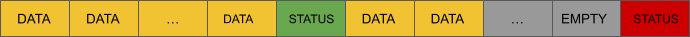
\includegraphics{figs/ringbuffer.png}
	        }
	    \caption{Ringbuffer}
	    \label{fig:ringbuffer}
	\end{figure}

\subsection{Writer}
The ring-buffer operates in two different modes, one is a `write' mode where the ring-buffer is used to relay information to another domain. In this mode of operation, writes occur by simply waiting for the status segment to be \mintinline{c}{BUFFER_WAITING}, this value indicates that the other domain is now waiting for input and therefore we can now write to the associated data segment of that specific cache line. For example, if we refer to figure \ref{fig:ringbuffer} we can see the writer in the process of filing up the data slots for the second cache line, after this has happened the status segment of the second cache line will be set to \mintinline{c}{BUFFER_READY} and therefore will be available for the reading domain to read from. 

\subsection{Reader}
As mentioned previously, the ring-buffer operates in two different modes, the `read' mode is how a domain is able to receive a message from another domain. Here, we simply wait till our status segment is set to \mintinline{c}{BUFFER_READY}, this value indicates that the writing domain has a cache line worth of information ready to be consumed by the reading domain. In this case, we read these values into a buffer and update the status segment to \mintinline{c}{BUFFER_WAITING}, which will allow the writer to reuse this memory again. 

\subsection{Memory Consistency}
One problem with how the ring-buffers work on ARM processors is that the ARM processors implement quite a weak form of memory consistency, in order to address this issue we had to add barriers before reading the status segments and barriers again before updating status registers. The barriers before the reading helped ensure that all memory was up to date and the barrier before updating ensured that all the read/write operations had propagated before the status was set.  

\section{UMP channel}
Our ringbuffer is a single writer, single reader data structure. Therefore, in order to support a two-way communication we employed two ringbuffers, one for each direction. We split a frame shared between the two communicating ends into two halves as shown on Figure \ref{fig:ump_panes}. Each half contains a ringbuffer. The first endpoint is a sender for one ringbuffer and a receiver for the other. The second endpoint, unsurprisingly, receives where the first sends and sends where the first receives.

\begin{figure}[ht]
    \centering
        \scalebox{0.8}{
            \includesvg{./figs/ump_panes.svg}
        }
    \caption{Using two ringbuffers to build a two-way UMP channel.}
    \label{fig:ump_panes}
\end{figure}

Alternatively, it would be possible to use a more sophisticated ringbuffer supporting multiple writers and readers. However, we found the approach with two ringbuffers much simpler.

In the initial implementation, the receiver explicitly polled the corresponding ringbuffer in a separate thread. For convenience, we later incorporated our UMP channel into \mintinline{c}{waitset} so that we could build an abstraction over UMP and LMP channels. Finally, to give 

\section{Sending capabilities and big messages}
To send messages of arbitrary sizes we use an encoding very similar to the one we used for LMP which just contains the buffer length in the header. To support sending frame capabilities between two  \mintinline{c}{init} domains, we also include enough information to forge the frame capability in the foreign \mintinline{c}{init}. Each UMP message is $56$ bytes long and we use the first message just for the header. Here's how it looks:

\begin{figure}[ht]
    \centering
        \scalebox{0.8}{
            \includesvg{./figs/ump_message.svg}
        }
    \caption{A general format of a message on a UMP channel.}
    \label{fig:ump_msg}
\end{figure}

The \mintinline{c}{frame.base}, \mintinline{c}{frame.bytes}, and \mintinline{c}{core_id} are used to forge a frame capability on the receiving end.

Also note that the full 56B are used for the header -- there's definitely room for an optimization. however as seen on the figure \ref{fig:ump_rtt} the RTT grows linearly with the message size (it's a log plot) so saving a single UMP message does not make a big difference. Therefore, we chose to keep things simple.

\subsection{Benchmarks}
\label{sec:ump_bench}

The Figure \ref{fig:ump_rtt} shows RTT scaling of our implementation of messages over UMP. First, it's important to notice that for small messages the difference to LMP is small (16B over LMP takes 26$\mu$s and over UMP 17$\mu$s\footnote{These numbers should be taken with a grain of salt because we just took an average of many runs so we don't know how the distribution looks.}). However, for big messages, UMP scales much better. We attribute this to the fact that since the communication is cross-core, the reader and writer can process data in parallel and no context switches are needed as opposed to the LMP.


\begin{figure}[ht]
    \centering
        \scalebox{0.8}{
            \includesvg{./figs/ump_really_big.svg}
        }
    \caption{Graph showing RTT of a single message over UMP across cores.}
    \label{fig:ump_rtt}
\end{figure}

\begin{hindsight}
Similarly to the implementation of arbitrary-sized messaged over LMP, we ended up quite satisfied with our UMP channels. But again, they didn't get to be fully appreciated because the RPC layer was our bottleneck by far. It would definitely be interesting to add a new "non-greedy" version of the UMP channels facilitating IPIs to see how big would be the performance hit.
\end{hindsight}

\section{All-to-all init UMP channels}
To avoid routing all communication through a single core, we added a UMP channel between each \mintinline{c}{init} domain in both directions (since our RPCs have a client-server structure). This means 12 UMP channels in total.

We achieve this by allocating a big enough frame on core 0 and passing this frame to each core's \mintinline{c}{init} through the \mintinline{c}{struct armv8_core_data}. The memory of each channel is predefined so each core knows how to initialize their channels.

It is of a bit hazardous as every ini\mintinline{c}{init} has access to every init-to-init UMP channel. There are of course safer approaches with better encapsulation, but we went for this implementation because of its simplicity. The channels turned out to be very useful, mostly for the Nameservice.

\section{A full binding system for arbitrary process-to-process communication}
\label{sec:full_binding_ump}

The code for this was deprecated and deleted since it was replaced by the name services.
We were providing the following interface:

\begin{minted}{c}
errval_t aos_rpc_create_server_on_port(struct aos_rpc_server_socket *server,
                                       uint16_t port);
errval_t aos_rpc_accept_connection(struct aos_rpc_server_socket *server,
                                   struct aos_rpc_client *socket);
errval_t aos_rpc_connect_to_port(struct aos_rpc_client *client,
                                uint16_t port);
\end{minted}

This allowed to any user process to create a server on a port. The port mapping was handled by a shared memory regions between all init processes on each core. This made it possible that a port can be acquired by using \mintinline{c}{atomic_cmpset_int()} and no other process was able to get the same port. Inside the port map the init would write its core s.t. other client that want to connect can contact the init on the right core to establish the connection. \mintinline{c}{aos_rpc_create_server_on_port()} created a LMP channel to the init on the same core that also acquired the port for us. \mintinline{c}{aos_rpc_accept_connection()} wait blockingly on that LMP channel waiting init to inform us about a client being connected.  \mintinline{c}{aos_rpc_connect_to_port()} will create a UMP frame send it to our init, which will forward the request to the owning core (by a lookup in the port map). The init on the owning core will then find the LMP channel for this port and send the UMP frame to the server waiting for it, this will unblock \mintinline{c}{aos_rpc_accept_connection} and return a connection to the other process.

(The commit hash of this was "43404b87930af75be8b2e0067d8e22b7fdc76d3d")
%nice
	\chapter{RPC}
\label{sec:rpc}

The LMP and UMP channels described in previous chapters can send arbitrary-sized messages and capabilities. Next, to build a basic RPC layer we need to:
\begin{enumerate}
    \item \emph{Abstract} away the two types of channels.
    \item \emph{Marshall} basic types (int, string, \ldots).
    \item Provide a framework for callers (clients) to call and for callees (servers) to handle the RPCs.
\end{enumerate}

We did not create a separate layer for the abstraction above the LMP and UMP channels, it is done inside \mintinline{c}{struct aos_rpc}. We also did not create separate structs for client and server, but \mintinline{c}{struct aos_rpc} can be initialized either as client or as a server.

\begin{minted}{c}
struct aos_rpc {
    enum aos_rpc_chan_type chan_type;

    union {
        struct lmp_chan lmp;
        struct ump_chan ump;
    } chan;

    // Mutex ensuring that at any point there's only at most one open rpc call.
    struct thread_mutex mutex;

    // Server-specific.
    struct waitset *ws;
    aos_rpc_eventhandler_t *eventhandler;
    void *server_state;
};


errval_t aos_rpc_init_lmp_server(struct aos_rpc *rpc, struct waitset *waitset,
                                 aos_rpc_eventhandler_t eventhandler, void *server_state);

errval_t aos_rpc_establish_lmp_client(struct aos_rpc *rpc, struct capref remote_ep);

errval_t aos_rpc_init_ump_server(struct aos_rpc *rpc, void *buf, size_t buflen,
                                 struct waitset *waitset,
                                 aos_rpc_eventhandler_t eventhandler, void *server_state);

void aos_rpc_init_ump_client(struct aos_rpc *rpc, void *buf, size_t buflen);
\end{minted}

A server registers with an eventhandler which is then called from the \mintinline{c}{event_dispatch(rpc->ws)}. Initially, there was no indirection and the user-provided eventhandler was the one directly registered with the \mintinline{c}{waitset}. Once we introduced Protobufs we also added an indirection to the eventhandler.
What follows is our RPC journey.

\section{Initial design}
At first we implemented a protocol more general than RPC. With RPC, a caller typically sends one message as a request and gets one message back as a response. Instead, we allowed arbitrary amount of messages between the client (caller) and server (callee).
This was because we didn't have a way of marshalling a full request/response, consisting of multiple arguments, into a single bytestream. So we could send an int, a string, etc, but only as separate messages.

Below code shows a \emph{very} simplified version of our initial designed (e.g., no error handling). It is the process-spawning RPC call.

\begin{minted}{c}
errval_t aos_rpc_process_spawn(struct aos_rpc *rpc, char *cmdline,
                               coreid_t core, domainid_t *newdid) {
    thread_mutex_lock(&rpc->mutex);
    
    // Send method.
    aos_rpc_send_method(rpc, AOS_RPC_METHOD_PROCESS_SPAWN);
    
    // Send arguments.
    aos_rpc_send_number(rpc, core);
    aos_rpc_send_string(rpc, cmdline);
    
    // Receive response.
    aos_rpc_recv_number(rpc, newdid);

    thread_mutex_unlock(&rpc->mutex);
}

errval_t aos_rpc_eventhandler(void *args) {
    struct aos_rpc *rpc = (struct aos_rpc *)args;
    thread_mutex_lock(&rpc->mutex);
        
    // Receive method.
    enum rpc_method;
    aos_rpc_recv_method(rpc, &rpc_method);
    
    switch (rpc_method) {
    case AOS_RPC_METHOD_PROCESS_SPAWN:
    {
        // Receive arguments.
        int core;
        char *cmdline;
        aos_rpc_recv_number(rpc, &core);
        aos_rpc_recv_string(rpc, &cmdline);
        
        // Send response.
        int newdid = handle_process_spawn(core, cmdline);
        aos_rpc_send_number(rpc, newdid);
    }
    break;
    }
    
    thread_mutex_unlock(&rpc->mutex);
}
\end{minted}

Funcionality-wise, this approach suffices for all use cases of this course. What's about to be shown in the rest of this chapter is basically us going on a great tangent :) However, a fun one, pinkie promise!

We didn't like two things about our initial design:
\begin{enumerate}
    \item For LMP, each \mintinline{c}{aos_rpc_send_*()} means a context switch to the receiving domain.
    \item The glue code for sending/receiving is error-prone and tedious to write.
\end{enumerate}

The first problem means quite a slowdown as we've seen in the benchmarks for LMP without SYNC optimization (\autoref{sec:lmp_sync_and_buf}). To remedy this, we could add a \mintinline{c}{should_sync} flag to each \mintinline{c}{aos_rpc_send_*()} or have a \mintinline{c}{aos_rpc_send_sync()} call that would SYNC and the rest of the calls would not. However, these solutions did not spark a lot of joy for us. The underlying issue really is that we can't marshall all arguments into one continuous message. In the next subsections we'll see how we, in our opinion very successfully, solved this by using Protobufs.

The issue of tedious glue code where each RPC call like \mintinline{c}{aos_rpc_process_spawn()} needs to be explicitly user-created is also rooted in the fact that we don't have an abstraction over sending arbitrary packed requests/responses. Here, we didn't push the Protobuf solution to its full potential so there's still quite some boilerplate that needs to be written. It's definitely more expressive, though.

\subsection{Marshalling using structs}
Our problem with marshalling would actually never exist if we just had to support types with memory requirements known at compilation time like ints. We would just create a struct containing the request parameters, interpret it as bytes, send the bytes over, and interpret the bytes on the other side as the struct again. However, this solution breaks with types like strings or more generally arrays which might have unknown memory requirements at compilation time.

\begin{minted}{c}
struct ProcessSpawnRequest {
    coreid_t coreid;
    char *cmdline;
};
\end{minted}

The example above illustrates this issue. The \mintinline{c}{char *cmdline} is just a pointer instead of actual bytes of the string inside of the \mintinline{c}{struct ProcessSpawnRequest}.

\section{Protobufs}
Instead of discussing more marshalling ideas we had we'll just jump to the conclusion: we couldn't come up with a simple enough design which would not require substantial amount of work. And a lot of work also means a lot of potential sources of bugs. Therefore, we incorporated an existing solution. Time-wise this is also a lot of work, but in the end less of our code and more of "battle-tested" code so more likely to JustWork\texttrademark.

Protocol buffers\footnote{https://developers.google.com/protocol-buffers/docs/proto3}, or Protobufs, is a language introduced by Google for serializing structured data. The user defines messages, services, and RPCs in a .proto file. For example:
\begin{minted}{proto}
// rpcs.proto
message ProcessSpawnRequest {
  uint32 core = 1;
  string cmdline = 2;
}

message ProcessSpawnResponse {
  uint32 pid = 1;
}

service ProcessService {
    rpc Spawn(ProcessSpawnRequest) returns (ProcessSpawnResponse);
}
\end{minted}

Using a library like \mintinline{c}{protobuf-c}\footnote{https://github.com/protobuf-c/protobuf-c}, hooks in C language for serializing/deserializing of the messages can be generated. Ideally, hooks for the services and the RPCs within it are generated as well. Then we would for example want the client interface to look as follows:
\begin{minted}{c}
#include <rpc_generated.h>

errval_t aos_rpc_process_spawn(char *cmdline, coreid_t core, domainid_t *newdid) {
    // Connect to the Process service.
    ProcessService ps;
    nameservice_lookup("process_service", (ServiceBase *)&ps);
    
    // Call the Spawn RPC.
    // Caller is responsible for cleaning up the request and response memory.
    ProcessSpawnRequest req = {
        .core = core,
        .cmdline = cmdline,
    };
    ProcessSpawnResponse res;
    errval_t err = ps->spawn(ps, &req, &res);
    PUSH_RETURN_IF(err, RPC_ERR_PROCESS_SPAWN);
    *newpid = res.pid;

    return SYS_ERR_OK;
}
\end{minted}

We omit the server interface of this ideal-world interface for brevity. We quickly realized that without modifying the \mintinline{c}{protobuf-c}, there's no way to get an interface this intuitive. Plus we would need to add a new "capability" type to the protos. We swallowed our pride and came up with a compromise described in the next subsection. We still leverage the serialization of Protobufs, but don't autogenerate RPC and service hooks. The serialization generated by \mintinline{c}{protobuf-c} has the following interface (excerpt containing the most interesting functions):
\begin{minted}{c}
// Initializes a message.
void   process_spawn_request__init
                     (ProcessSpawnRequest         *message);
// Serializes a message into `out` buffer.
size_t process_spawn_request__pack
                     (const ProcessSpawnRequest   *message,
                      uint8_t             *out);
// Deserializes a serialized message.
ProcessSpawnRequest *process_spawn_request__unpack
                     (ProtobufCAllocator  *allocator,
                      size_t               len,
                      const uint8_t       *data);
\end{minted}

\subsection{The integration}
Here is the final interface we use that did not require changes in the \mintinline{c}{protobuf-c} autogeneration:
\begin{minted}{proto}
enum RpcMethod {
  PROCESS_SPAWN = 0;
  
  // DO NOT CHANGE: Setting up LMP channels depends on this value being 9.
  SEND_LOCAL_LMP_EP = 9;
}

// ProcessSpawnRequest and ProcessSpawnResponse omitted.

message RpcRequestWrap {
  oneof data {
    ProcessSpawnRequest process_spawn = 2;
  }
}

message RpcResponseWrap {
  uint64 err = 1;

  oneof data {
    ProcessSpawnResponse process_spawn = 2;
  }
}

message RpcMessage {
  RpcMethod method = 1;

  oneof direction {
    RpcRequestWrap request = 2;
    RpcResponseWrap response = 3;
  }
}
\end{minted}

"On the wire" we always send around the \mintinline{c}{RpcMessage} so that we always know which message type to deserialize the received bytes into. The \mintinline{c}{RpcRequestWrap} and \mintinline{c}{RpcResponseWrap} are used on the client-side as follows:
\begin{minted}{c}
// Calls an RPC `method` with `request` payload and `request_cap` capability. Receives the
// response payload in callee-allocated `response` and response capability in `response_cap`.
// In case of an error (remote or local), returns the corresponding error code.
errval_t aos_rpc_call(struct aos_rpc *rpc, RpcMethod method, RpcRequestWrap *request,
                      struct capref request_cap, RpcResponseWrap **response,
                      struct capref *response_cap);

errval_t aos_rpc_process_spawn(struct aos_rpc *rpc, char *cmdline, coreid_t core,
                               domainid_t *newpid) {
    ProcessSpawnRequest req = PROCESS_SPAWN_REQUEST__INIT;
    req.core = core;
    req.cmdline = cmdline;
    // A macro that creates RpcRequestWrap with the `req`. The lowercase "init_process_spawn"
    // and uppercase "INIT_PROCESS_SPAWN" are needed for the field names in the macro.
    REQUEST_WRAP(req_wrap, init_process_spawn, INIT_PROCESS_SPAWN, &req);
    
    RpcResponseWrap *res_wrap = NULL;
    aos_rpc_call(rpc, RPC_METHOD__PROCESS_SPAWN, &req_wrap, NULL_CAP,
                       &res_wrap, NULL);
    
    *newpid = res_wrap->process_spawn->pid;
    // Destroy the callee-allocated response payload.
    RESPONSE_WRAP_DESTROY(res_wrap);

    return SYS_ERR_OK;
}
\end{minted}

The interface is far from the ideal shown before, but it's okay to justify the fact that now we can send requests and responses containing almost arbitrary data (ints, strings, arrays, nested proto messages, arrays of nested proto messages, you name it!).

Under the hood, the \mintinline{c}{aos_rpc_call()} puts the \mintinline{c}{request} into \mintinline{c}{RpcMessage} with the corresponding \mintinline{c}{method} and sends this serialized to the other endpoint. Then it receives a response \mintinline{c}{RpcMessage}, deserializes it and takes out the \mintinline{c}{RpcResponseWrap} to return it to the sender. 

What remains is to discuss how this is handled on the server side. There's not much magic to it -- the global handler registered with the waitset takes out the \mintinline{c}{RpcRequestWrap} from the received \mintinline{c}{RpcMessage}, preallocates a response and calls the user-provided handler. The handler fills the response which is then put into \mintinline{c}{RpcMessage} and send to the caller.

\section{Benchmarks}
When running our RPC benchmarks over both UMP and LMP we observed that every RPC took roughly 80ms. That's basically an eternity because we were expecting a single call to be in the order of microseconds. This was the case even for the smallest messages of sizes 16B. At first, we thought the Protobuf serialization is slow, but when microbenchmarking it separately it ran in microseconds.

Then we looked closely at the UMP case. We found out that time between a message being added to the buffer and the time when the domain receiving the buffer was scheduled, was almost 80ms. The receiving domain seems to be scheduled very sparsely when using the active polling in the \mintinline{c}{waitset}. Note that  the same issue was observed in the Network implementation and led to a separate active polling thread implementation, see \autoref{net:high_speed}.

One can now wonder why did the issue not appear in the "raw" LMP/UMP benchmark in \autoref{sec:ump_bench}. Therefore, we went back to these benchmarks and tried to make them a little slower "simulating" what happens in the RPC case. Our suspicion was that the issue has to do with scheduling. And in line with this believe is that when adding a \mintinline{c}{barrelfish_usleep(400)} right before sending the data over for the "raw" LMP/UMP, the RTT takes 80ms (as opposed to an expectation of say at most 10ms) given that the sleep function has takes microseconds as argument. 

Since this slowdown affects every individual project, we put serious effort into finding the root cause, but unsuccessfully. Our suspicion is that it's an issue in the scheduler.

\subsection{Elimination of memory copies}
\label{sec:rpc_proto_opt}
The Protobuf layer currently incurs two memory copies when receiving: one to receive data from the underlying channel (LMP/UMP) and another to deserialize the data. Analogously for sending.

This can be brought down to just a single memory copy -- when copying data to and from the underlying channel. The \mintinline{c}{Protobuf-c} has support for this, but since our bottleneck ended up being the 80ms bug, we didn't implement this optimization. 

\begin{hindsight}
Overall, we think it was a good idea to overengineer the RPCs a little. The API turned out okayish, causing occasional headaches, but concise enough for most cases. Compared to the initial design which required writing glue code ourselves, we went from trusting some ("battletest") glue codes to trusting all of them because they were generated. 

The biggest takeaway though is to benchmark early. We only discovered the 80ms bug three days before the deadline. And sadly, we were not able to identify the root cause in time despite putting in decent hours.
\end{hindsight}
	\chapter{Shell}
Since only a single process can write to the serial output, some extra engineering effort was required to ensure this property was maintained while still not majorly impacting how the libc's standard functions worked. 

\section{Terminal Service}
The shell along with other processes on the system are configured to make RPC requests to the terminal service in order to interact with the UART device. This involved using the nameserver to register a service along with an appropriate handler function to handle terminal related RPC requests. 

\subsection{User space UART}
For the user space UART to work, the terminal service expects a device capability to the UART device being mapped into one of the argument capability slots. We use the \mintinline{c}{map_device_register} function along with the relevant memory location data to map the device frame into our virtual address space. From here it is as simple as calling the \mintinline{c}{lpuart_init} function to initialise the driver. 

\subsection{Interrupts not delivered}
Unfortunately, despite correctly (at least seemingly) configuring the GIC and the user space UART, we were unable to receive interrupts. In order to address this, we had to re-evaluate how input would work, the solution we eventually ended up going with was to simply read in a busy loop for input. While this did solve our problem, it did unfortunately introduce a large performance penalty. 

\subsection{Multiplexing Input/Output}
Multiplexing output was quite trivial due to how we implemented the printf functionality. Whenever we received a whole string, we simply printed that out. This does mean that it is possible for a foreground domain to mangle output, however this is a user level error. Multiplexing input was however much harder. We achieved this through locks as described in the session management section \ref{sec:sessions}.

\subsubsection{Session management}
\label{sec:sessions}
As mention previously, it is critical that only a single process owns access to the serial input interface. In order to achieve this we explored several venues such as allocating the UART device to a single process until a newline character has been read. However, in order to give the caller more control, we provided a method to lock and release a lock used to indicate ownership of the UART interface's read capability.

\subsubsection{Lazy terminal initialisation}
Unfortunately, due to constraints where (chronologically) the libc glue code was initialised we were not able to obtain a terminal instance and directly connect the IO functions. In order to provide a solution for this, we implemented a lazy loading of the terminal service. This was achieved by delaying the connection attempt till after a user space write/read call was made. 


\section{Shell}
The shell itself is quite simple and is just a wrapper over the terminal. It of course does allow for process spawning and other shell related functionality. For the shell, we implemented a custom recursive descent parser in order to parse commands, although in hindsight such a parser is likely overkill. From this point onward, we simply do a `strcmp' for each available command and simply call the appropriate function.  

\section{Improvements}

\subsection{UART as a capability}
Given the nature of Barellfish and its existing capability system,  it does make sense to have a capability type for the serial input/output interface. This not only makes sense from an ergonomic perspective but may help deter the current existing attack vectors. For example, currently a process is capable of faking it's pid in the request to the terminal service. This is obviously not the desired behaviour. Unfortunately, due to the complexity of the capability system we did not want to explore how to implement such a capability since we had other time pressing issues.

\subsection{First Come/First Serve}
The consequence of having the lock on the serial interface means that a single process can hold onto the interface for an extended period of time. Unfortunately there are no solutions here to multiplex this better outright. The various other solutions require tradeoffs and we
decided that the tradeoff offered via this central locking scheme was more attractive than other multiplexing methods, for example such as a newline character for example.	
% 	\input{capabilities.tex} 
	\chapter{Filesystem}

This chapter discusses the filesystem project.
We will first analyze the performance of the provided block driver and consider
a simple optimization.
Then we lay out the design of the Filesystem infrastructure that we built on top
of this driver discussing each component in detail.

\section{Block Driver Performance}

As the book states, the provided block driver is incredibly slow.
As seen in \autoref{fig:fs_sdhc} the provided driver takes 953.55ms to read and
960.01ms to write a block from or to the SD card.
These measurements were done by repeatedly (30 times) transferring a block (512 Bytes) between a sector on the device and a fixed physical address on the host.
Reading and writing were measured separately.
This was tested with both the provided SD card as well as a model from SanDisk.
Both yielded comparable results, so that we only show the former since it was provided by the course.

Note, that this benchmark was performed while the full OS was running.
It was also executed on core 0, where most services -including the filesystem server- run.
These measurements thus represent a more realistic scenario than an isolated 
benchmark since it also measures interference from, for example, the scheduler.
This shows the performance impact of the various \mintinline{C}{barrelfish_usleep}
operations that the driver performs since these will result in yielding the
calling process.

When talking to other teams, we discovered that their baseline was more in the
range of 450ms. They appeared to be measuring performance in a more isolated setting.
While this is good for obtaining the best case performance of the driver, 
the results of our benchmark show the added performance impact of yielding in
the setting of a contested scheduler.

\begin{figure}[ht]
    \centering
    \scalebox{0.6}{\includesvg{./figs/fs_sdhc.svg} }
    \caption{SDHC Block driver performance with and without our optimization.}
    \label{fig:fs_sdhc}
\end{figure}

There is plenty of potential for speedup here, since modern SD card can reach transfer-speeds of multiple MB/s. 

We were restricted on time and thus chose not to explore the optimization of the
driver in great detail.
Instead we focus on the engineering challenge of creating a filesystem around the block device.
The filesystem will have to try to mitigate the performance impact of the slow driver.

However, We did find a small optimization that results in a roughly $2x$
speedup.

Looking at the implementation of \mintinline{c}{sdhc_read_block} and \mintinline{c}{sdhc_write_block} we noticed that a set block length command is send before every read and write.
This seemed redundant since the block length does not change during the
execution.
Removing these commands resulted in a read latency of 473.54ms per block and a
write latency of 480ms per block.
We still issue the command to set the block size once at the beginning when initializing the device.

The question remains whether this is a legitimate optimization or if we are sacrificing correctness and conformity to the protocol by doing this.
After extensive testing we did not encounter any errors when transferring blocks and thus assume that this optimization is legitimate. 

The benchmark for the block operations can be found in \mintinline{c}{usr/drivers/fsfat32/benchmarks/sd_card_bench.h}

In the following we will assume the block driver runs with our optimization.

\section{FAT32 Filesystem}

As suggested in the courses accompanying book we implement a filesystem for FAT32 formatted block devices.
The implementation tries to be close to the standard, but cuts some corners to save time.
The filesystem infrastructure consists of multiple layers that provide increasingly abstract interfaces for reading and writing to the FAT32 formatted block device.

These components are, in increasing abstraction:
\begin{itemize}
    \item An \textit{SDHC Wrapper} Library around the provided driver.
    \item A \textit{FAT32 Library} for basic file operations.
    \item A \textit{Filesystem Server} providing an RPC interface to the files and controlling access to the same.
    \item A \textit{Client Side Library (fatfs lib)} to interact with the RPC Server and maintain the state of files in the client.
\end{itemize}

Figure \ref{fig:fs_arch} gives an overview of the Architecure of the Filesystem
infrastructure.
In the following we will discuss these components in detail.

\begin{figure}[ht]
    \centering
    \scalebox{0.6}{\includesvg{./figs/FSServer_Infra.svg} }
    \caption{Architecture of the Filesystem Infrastructure.}
    \label{fig:fs_arch}
\end{figure}


\subsection{SDHC Wrapper}

The provided driver only exposes an interface for transferring single blocks between the device and a physical memory location.
Using this interface directly is clumsy which is why we create a wrapper around it. 
This wrapper provides functions for reading and writing multiple blocks and just parts of blocks to either physical or virtual addresses:

\begin{minted}{c}
errval_t read_from_sd_offset(struct sd_wrapper *sd, void *dst, uint32_t sector, 
                                uint32_t offset, uint32_t size);
errval_t write_to_sd_offset(struct sd_wrapper *sd, uint32_t sector, 
                                uint32_t offset, const void *src, uint32_t size);

errval_t read_from_sd_to_paddr(struct sd_wrapper *sd, lpaddr_t paddr, 
                                uint32_t sector, uint32_t size);
errval_t write_to_sd_from_paddr(struct sd_wrapper *sd, lpaddr_t paddr, 
                                uint32_t sector, uint32_t size);
\end{minted}

The first two functions allow reading and writing data of arbitrary sizes at any offset withing a block.

We will use the terms sector and block interchangeably. For both we assume 512 bytes.

When using \mintinline{C}{read_from_sd_offset()}, the block driver writes to an internal buffer. 
The desired chunks are then copied over to the buffer provided by the user.
Writing works analogously.

The latter two calls do not buffer and thus require less copying. 
This results in them being slightly more restrictive, as they do not allow an offset and the size parameter has to be a multiple of the block size.

\subsubsection{Idea for Optimization: Caching Blocks}
As described later in the chapter, we already have a write-through cache for FAT entries.
When writing back the entries, this uses the buffered operations provided by this wrapper.

By using a write-back cache, we could further cache the write accesses in the buffer and only write them to disk, when we need the buffer space for something else.
This would eliminates a lot of accesses to the device, since usually (assuming locality) fat entries are grouped together.

This could also be useful when iterating through directories.

It is probably less useful for writing and reading large chunks of data. The
cache will constantly be evicted by the next chunk.

This is currently not implemented, but might be an interesting investigation for
future work.

\subsection{FAT32 Library "usr/drivers/fsfat32/fat32\_file\_system.h"}

Our FAT32 provides the functionality to lookup, create, read, and modify both files and directories.
It exposes the following API:

\begin{minted}{c}
// Create and Delete Files or Directories.
errval_t fat32_create_file(struct fat32_file_system *fat, struct dir_entry *parent,
                            char *name, uint8_t attr, struct dir_entry *ret);
errval_t fat32_delete_file(struct fat32_file_system *fat, struct dir_entry *parent, 
                            struct dir_entry *dir_entry);

// Read / Write / Append files.
errval_t fat32_read(struct fat32_file_system *fat, struct dir_entry *dir_entry,
                            void *buf, size_t pos, size_t bytes, size_t *ret_bytes);
errval_t fat32_write(struct fat32_file_system *fat, struct dir_entry *dir_entry,
                            void *buf, size_t pos, size_t bytes, size_t *ret_bytes);

// Uses read_from_sd_to_paddr to directly read the entire file into a frame.
errval_t fat32_readfile_to_frame(struct fat32_file_system *fat, struct dir_entry *dir_entry,
                                struct capref frame, size_t *ret_bytes); 
// Truncate a file.
errval_t fat32_trunc(struct fat32_file_system *fat, struct dir_entry *dir_entry, size_t bytes);

// Find a file or directory by path.
errval_t fat32_resolve_path(struct fat32_file_system *fat, const char *path,
                            struct dir_entry *result);
// Find a file or directory in parent by name.
errval_t fat32_find_dirent(struct fat32_file_system *fat, struct dir_entry *parent,
                            char *filename, struct dir_entry *res);


// Finds the position and name of the next non-empty directory entry in parent after the given offset.
// Return FS_ERR_INDEX_BOUNDS if the end of the directory is reached.
errval_t read_next_dir_after_offset(struct fat32_file_system *fat, struct dir_entry *parent,
                                    uint64_t offset, char **ret_name, uint64_t *ret_idx);
\end{minted}

Files and directories are represented as dir\_entry structures which contain a copy of the FAT32 directory entry as well as the position of the directory entry on the disk.
In general, files and directories are treated interchangeably. 
They can be distinguished by the directory bit in the attribute entry.

Not all operations are allowed on both directory entry types and will return FS\_ERR\_NOTFILE or FS\_ERR\_NOTDIR as appropriate.
In general, lookup (find/resolve), creation, and deletion are defined for both.
Reading, writing, and truncating are only allowed on files.
To iterate through directories, we provide read\_next\_dir\_after\_offset.

Note that the create function will not check if a file or directory with that name already exists.
This must be checked by the caller beforehand.

Delete will only remove directories if they are empty.
We do not provide a direct interface to recursively delete a directory, since the function would have to check if files are still being used.
This is out of scope for this layer (In fact, this is completely left up to the end user of the library).

This layer notably provides an offset based layer.
Streaming functionality must be implemented on top.
Unfortunately, this means that, for every operation, files have to be traversed from the beginning until the specified offset is reached.
We made this choice to reduce the amount of state that has to be kept by the filesystem server.
A streaming API would require the server to keep track of the position in the file for every user that opens it.
Keeping in line with the design of Barrelfish, we instead outsource this responsibility to the user.

This design means that fast access to the file allocation table is critical.
We achieve this using a fat cache.

\subsubsection{Optimization: File Allocation Table Cache}
Originally, all operation in the library would read and write to the block device to obtain data.
Every read and write to an entry entry in the file allocation table resulted in a complete block operation to the SD card.
This meant that traversing files was slow.

To solve this we simply cache the file allocation table in memory.
This speeds up file traversal significantly. 

Figure \ref{fig:fs_read_one} shows the latency of reading a single cluster (4096Bytes) with a cached FAT entry vs a non cached FAT entry.


\begin{figure}[ht]
    \centering
    \scalebox{0.6}{\includesvg{./figs/fs_read_one_cluster.svg} }
    \caption{}
    \label{fig:fs_read_one}
\end{figure}

% uncached read ms     2144.038829
% cached read ms    1920.049408

However, since reading from the SD Card is prohibitively slow it is impractical to read the entire file allocation table upon startup.
This would mean a significant delay when starting up the system.
It is also most likely unnecessary since not all FAT entries are needed right away. 

Instead we load the FAT on demand.
Whenever a non cached entry is read, we read the entire cluster containing the FAT entry into the cache.
To keep consistency between the cache and the block device we use the write-through strategy.
This means that updating a FAT entry results in writing the surrounding block to the block device.
As a result, updating a fat entry is still expensive, but there is a noticeable difference reading is significantly faster.

\subsubsection{Performance}

For brevity, we evaluate the performance of a subset of the provided operations.
We measure each execution 30 times and report the median.
The variance is shown using small bars, but is usually so negligible that it is
not visible.

\begin{figure}[ht]
    \centering
         \subfloat[\centering ]{{\scalebox{0.4}{\includesvg{./figs/fs_fat32_lib_ops.svg} }}}
         \subfloat[\centering ]{{\scalebox{0.4}{\includesvg{./figs/fs_fat32_lib_ops_slow.svg} }}}
    \caption{}
    \label{fig:fs_fat32_lib_ops}
    
% creation_ms                      2.391705
% append_ms                        2.888078
% find_ms                          0.240011
% deletion_ms                     31.680818
% reading_large_file_ms_40961B    19.444631
\end{figure}

Figure \ref{fig:fs_fat32_lib_ops} clearly shows the limitations of the block
driver.
Finding a file in a short directory, creating a file, and appending to an empty
file are all relatively fast at $0.24ms$, $2.39ms$, and $2.89ms$ respectively.
All of these instructions need a limited amount of block operations.

Deleting and reading a large (40kB) file are considerably slower with $31.68ms$
and $19.44ms$.
These require more interaction with the block device.
Deleting a file takes such a long time because the operation tries to cleanup
the parent directory to release potentially empty clusters.
This must be done to prevent the SD card running out of capacity without
actually storing any data. 


\subsection{Filesystem Server "usr/drivers/fsfat/"}

The filesystem server exposes file operations using an RPC interface.
It exposed interface can be found through the nameservice by looking up "FS/<mountpoint>".
Since we only provide the filesystem for the SD card, we set this to be "FS/sdcard".

This allows multiple filesystems to be mounted as a sort of VFS.
This is currently, however, not supported by the client side library.

The filesystem exposes the following RPC calls:
\begin{minted}{c}
FS_OPEN                 // (path, flags) -> fd, size
FS_CREATE               // (path, flags, is_dir) -> fd
FS_CLOSE                // (fd) -> void
FS_READ                 // (fd, offset, size) -> data
FS_WRITE                // (fd, data, offset) -> size
FS_TRUNC                // (fd, size)
FS_OPENDIR              // (path) -> fd
FS_READNEXTDIR          // (fd, pos) -> filename
FS_DELETE               // (path) -> void       - Used for file & dirs
FS_READFILE_TO_FRAME    // (fd, frame_cap) -> size
\end{minted}

Like the FAT32 library that backs these RPC calls, the position in the file is
specified using offsets from the beginning of the file.

As the central point for file access to the mounted device, the server must ensure that two invariants are upheld.
Firstly, there must never be more then one simultaneous read issued to the underlying block device.
Secondly, write access to a file must always be exclusive while read accesses may overlap.
These are needed to guarantee the consistency of the filesystem.

The first invariant is trivially upheld, since the server handles all incoming requests sequentially in a single "event handler loop".

To ensure the second invariant, the server tracks which files are opened and
with which permissions.
For a client, trying to open a file, this means the following:
If the client wants to open the file with write permissions, it is only granted
access if the file is not currently opened.
If the client wants to read the file, the file must not already be opened with
write permissions.
Note, that the server does not keep track which processes have opened files or
where in the file they are. 

There can be multiple readers at a time, the server keeps track of the number of
readers accessing it, so it knows when the file is not being accessed anymore.
The following snippet shows the just described handle kept by the server:

\begin{minted}{c}
struct file_handle {
    char *path;
    struct dir_entry dir_entry;
    uint32_t num_accessors;
    bool has_writer;
};

struct server_state {
    bool up;
    struct fat32_file_system fat;
    collections_hash_table *open_files;  // A hash table of FD -> file_handle
};
\end{minted}

\subsubsection{File Descriptors}
The avid reader might have noticed that the RPC interface presented above uses
file descriptors to identify files:
Opening a file will return a file descriptor which then has to be passed back as
arguments for other operations on that file.

The server uses this file descriptor to find the file\_handle in its internal
table.
Since there should only every be at most one handle per file, the file
descriptor that is handed out is deterministically calculated from the file
name.
It is calculated as an SDBM hash of the full file path.
Collisions are resolved by comparing the file names and sequentially checking
each increasing hash value.

As a side-effect, this allows for fast lookup for file operations.

\subsubsection{Drawbacks}
However, it also has a significant drawback:
Since file descriptors are deterministic a malicious process could access a file
that was opened by another process without actually having to open it itself by
computing the file descriptor using the hash function.

This would easily circumvent the single writer policy that the server tries to
enforce.

A solution for this would be to hand out capabilities which then contain the
hash to identify the file.
Since Barrelfish uses capabilities for most things, this method would integrate 
well with the existing ecosystem.

We leave it as future work, since it was not in the scope of this project.

\subsubsection{No SD detected}
When the filesystem server is started it will try to access and setup the block
device. If this succeeds, it then registers itself as a nameservice and responds
to queries as described in this chapter.

If the setup does not succeed, because, for example, there is no SD card
present, the fileserver will still register itself with the nameservice system
and respond to queries.
However, it will respond to all queries with the error code FS\_ERR\_NOT\_FOUND.

This mechanism is a placeholder, since the client library will always try to 
connect to filesystem server upon setup.

One alternative solution would be for the client to try to connect a fixed 
number of times and then fail if it could not connect.
This is unreliable and leads to unnecessary latency when starting a new process.

A better solution would be to provide another service that maintains a list of
mounted file servers (essentially providing a VFS).
The filesystem servers would then register with this service when it successfully
set up.
And the client would query the "VFS" server to obtain the list of mounted
file systems.


\subsection{Client Side Library "fs/fatfs.h"}

The client side library forms the glue between the general libc library and the
RPC filesystem server.

Upon initialization the client library will establish a connection to the
filesystem server for "/sdcard".
The library exposes a virtually identical interface to the ramfs library on which 
it is based and provides a C wrapper for the servers RPC interface.
It exposes the following interface to libc:

\begin{minted}{c}
errval_t fatfs_open(void *st, const char *path, int flags, fatfs_handle_t *rethandle);
errval_t fatfs_create(void *st, const char *path, int flags, fatfs_handle_t *rethandle);
errval_t fatfs_remove(void *st, const char *path);
errval_t fatfs_read(void *st, fatfs_handle_t handle, void *buffer, size_t bytes,
                    size_t *bytes_read);
errval_t fatfs_read_file_to_frame(fatfs_mount_t st, const char *path, struct capref frame, size_t *bytes_read);
errval_t fatfs_write(void *st, fatfs_handle_t handle, const void *buffer, size_t bytes,
                     size_t *bytes_written);
errval_t fatfs_truncate(void *st, fatfs_handle_t handle, size_t bytes);
errval_t fatfs_tell(void *st, fatfs_handle_t handle, size_t *pos);
errval_t fatfs_stat(void *st, fatfs_handle_t inhandle, struct fs_fileinfo *info);
errval_t fatfs_seek(void *st, fatfs_handle_t handle, enum fs_seekpos whence, off_t offset);
errval_t fatfs_close(void *st, fatfs_handle_t inhandle);
errval_t fatfs_opendir(void *st, const char *path, fatfs_handle_t *rethandle);
errval_t fatfs_dir_read_next(void *st, fatfs_handle_t inhandle, char **retname,
                             struct fs_fileinfo *info);
errval_t fatfs_closedir(void *st, fatfs_handle_t dhandle);
errval_t fatfs_mkdir(void *st, const char *path);
errval_t fatfs_rmdir(void *st, const char *path);
errval_t fatfs_mount(const char *uri, fatfs_mount_t *retst);
\end{minted}

Since the server does not track the position of the cursor for each process, the
client library has to do this itself.
It keeps a list of file handles that contain basic information about the files.
This includes, the position of the cursor and the filesize.
The client library is responsible for updating its own view information when
modifying the file.
This does not introduce consistency problems, since there can only ever be one
writer per file at a time (provided there is no malicious actor as described
above).
As a result, operations like fstat, fseek, and ftell do not require an RPC.
The filesystem server only needs to be accessed to open and close files or to
access information that is on the block device.

\subsection{Performance of the complete stack}

Finally, we want to take a look at the end to end performance of issuing a
filesystem operation from userspace.

We run the benchmark from a userspace program that is spawned after the filesystem server is set up.
All measurements were run 30 times with a complete running OS.
Append and read both operate on the first cluster (4KiB) of a file.

\begin{figure}[ht]
    \centering
    \scalebox{0.6}{\includesvg{./figs/fs_fat32_e2e.svg} }
    \caption{Performance of calling libc file operations: fopen, fwrite, fread, fclose}
    \label{fig:fs_libc_e2e}
% open_ms      5494.123975
% append_ms    8656.162013
% read_ms      3840.110825
% close_ms        0.050854
\end{figure}

The results of this benchmark can be seen in figure \ref{fig:fs_libc_e2e}.
We only inspect the most prominent operations for the sake of brevity.

Opening a file takes $5494.12ms$, this is due to the fact that the call also needs to create the file.
The implementation of fopen first checks if the file exists by trying to open it.
When this fails, because the file does not exist yet, it triggers another RPC to create the file.
This explains the additional delay compared to the direct create operation.

Appending the first block to a file file takes $5494.12ms$, which includes communication overhead and traversing the directory to obtain the file handle.
It is important to note, that libc does not try to write the entire cluster in one attempt. 
Instead it breaks it into 1024 byte chunks and triggers RPCs for each.
This explains the added overhead over the direct FAT32 Library call.

Reading is subjected to the same chunking. It thus also introduces overhead resulting in a median latency of $3840.11ms$.

Closing a file multiple orders of magnitude faster at $0.051$ since it does not require any block operations.
It is just a lookup in a hashmap and an RPC.


\section{Limitations}
As can be seen in this chapter, there are still some limitation to our implementation
\begin{enumerate}
    \item The block driver is still incredibly slow
    \item Loading ELF binaries is not implemented yet, binaries are quite large and would take an unacceptably  long time to load
    \item Anything that modifies FAT entries is slow, since the block is written back every time an entry is modified.
    \item We do not support timestamps.
    \item The access control is very limited. Integrating it with the capability system would be desirable.
    \item We currently do not support long names.
    \item Currently every file open is interpreted as a write, we would just need to add flag parsing to allow simultaneous reads.
    \item Open files are not automatically closed when the process dies.
\end{enumerate}

	\chapter{Nameservice}
I want to preface this chapter with the fact that the naming I chose is a bit unfortunate. By "Nameserver" I mean a name resolution service. By Nameservice I mean a layer that glues together the name resolution and service binding.

I went for a very simple solution where the Nameserver resolves a Service name (string) into a SID (Service ID). The SID uniquely identifies a service and can be used for routing capabilities through \mintinline{c}{init} because it encapsulates Core ID and Domain ID. In a DNS analogy the Service name is the domain name and SID is an IP.

I didn't implement extra challenges, but instead revamped the LMP/UMP/RPC stack and provided support for my teammates who started using the Nameservice early on, implementing their feature requests and debugging if needed.

\section{Connecting domains}
The first part of the Nameservice functionality is to allow connecting client and service domains via an LMP/UMP backed RPC channel.

\subsection{Existing work (ports)}
As mentioned before in section \ref{sec:full_binding_ump}, we had an implementation of primitive "service binding" even before the individual projects started. Each service operated on a unique "port" (int) and clients could bind to it over UMP, even cross core.

This required an extra routing table from ports to DIDs (Domain IDs) such that \mintinline{c}{init}s would know where to route the binding request. Later I show how I got rid of the ports to remove one indirection. This is because the Nameservice with the ports would have in total 3 indirections (Service name -> Port -> DID). I wanted to simplify this.

\subsection{The need for sending capabilities}
I wanted to connect intra-core client-service pairs via LMP and inter-core via UMP. UMP could be used for both cases, but even though I didn't benchmark this, LMP should be intuitively faster intra-core than UMP because sending messages intra-core is the LMP's very purpose.

Supporting the LMP connection creating is easy because sending capabilities over LMP is already supported. The client, however, does not necessarily have an existing connection to the service. So in order to exchange the client-service endpoint capabilities, we need to route through a common node, e.g., core's \mintinline{c}{init}.

For UMP, one endpoint (client) needs to allocate the frame for the channel and send it over to the other endpoint (service). One idea would be to just send frame information like base address and size, and forge it on the receiving end. However, only \mintinline{c}{init} can forge a capability.

There are a few approaches for designing a binding scheme with support for sending capabilities as described above. The one I found the most simple is shown on the figure \ref{fig:ns_network}.  

\begin{figure}[ht]
    \centering
        \scalebox{0.6}{\includesvg{./figs/ns_network.svg}}
    \caption{The network design of sending capabilities for connection requests.}
    \label{fig:ns_network}
\end{figure}


We see a \mintinline{c}{client} and \mintinline{c}{serviceA} on the same core 0. To connect to this service, the client sends its LMP endpoint over \mintinline{c}{init} to the \mintinline{c}{serviceA}. Afterward, this service finishes the binding via sending its remote connection, now directly to the client.

For an inter-core of \mintinline{c}{client} to \mintinline{c}{serviceB}, the client allocates a frame to back the new UMP connection. Then they send it over to \mintinline{c}{serviceB} via core 0 \mintinline{c}{init} and core 1 \mintinline{c}{init}.

There are two issues that need to be resolved. First, how does the \mintinline{c}{init} know over which channel to forward the capability. Second, the RPC channels from \mintinline{c}{init} to children domains don't exist yet. Remember that our RPC channels are unidirectional and the channels we set up on process spawn are from child to init.

\subsection{Service ID}
\label{sec:serviceid}
For routing, we assign each service a unique SID (Service ID) which contains its Domain ID and Local Service ID. The Domain ID itself consists of Core ID and Local Domain ID\footnote{Now that I'm writing this, maybe I could've picked the names a bit better.}. How this this organized in memory is shown on figure \ref{fig:ns_serviceid}.
\begin{figure}[ht]
    \centering
        \scalebox{0.6}{\includesvg{./figs/ns_serviceid.svg}}
    \caption{The definition of \mintinline{c}{serviceid_t} type.}
    \label{fig:ns_serviceid}
\end{figure}

The reason for not just using the Domain ID is that there can be multiple services in a single domain, hence Local Service ID.

A shortend form of the SIDs with the Local Service ID omitted can be seen on figure \ref{fig:ns_network} under domain names. Now using SIDs in the requests as destinations, \mintinline{c}{init} will always know to which domain to forward the request.

\subsection{\mintinline{c}{init} to domain channels}
Whenever a service gets registered, the \mintinline{c}{init} needs to be able to forward requests to it. Therefore, I lazily (only on the first call of \mintinline{c}{nameservice_register()} from a domain) establish a connection to \mintinline{c}{init} via an RPC method \mintinline{c}{INIT_ESTABLISH_DOMAIN_SERVER}. The important caveat here is that before establishing this connection, I spawn a thread which listens on the default waitset to be able to accept the connection. There are definitely nicer ways around this, but refactoring it ended up being a TODO :)

\subsection{A Route proto}.
During the design my teammates kept asking me if they'll be able to send frame capabilities arbitrarily over the nameservice channels. So instead of making a simple \mintinline{c}{ServiceConnect} RPC with arguments like this:
\begin{minted}{proto}
message ServiceConnectRequest {
  int64 destination_sid = 1;
  
  enum Type {
    UMP = 0;
    LMP = 1;
  }
  Type type = 2;
}
\end{minted}

I created a generic \mintinline{c}{Route} RPC which can route arbitrary request over the \mintinline{c}{init}s, thus allowing to send/receive capabilities with any request over nameservice channel. The request gets always routed directly, unless the underlying channel is UMP and we're sending/receiving capabilities.
\begin{minted}{proto}
message RouteRequest {
  uint64 destination_sid = 1;

  RpcMethod method = 2;
  RpcRequestWrap inner_request = 3;
}
\end{minted}

Then for example for a \mintinline{c}{ServiceConnectRequest}, I put it into the \mintinline{c}{RouteRequest} and send it over. Note that the \mintinline{c}{ServiceConnectRequest} then doesn't need to contain the \mintinline{c}{destination_sid} because the layer above, \mintinline{c}{RouteRequest}, has it.

\section{Avoiding deadlocks without async support}
The "routing" looks nice on the diagrams, but in reality these are nested RPC calls... This means that if we're dispatching on a single \mintinline{c}{waitset} in \mintinline{c}{init}, a deadlock is always lurking around the corner. Imagine for example all RPC channels being registered on the same waitset in each  \mintinline{c}{init}. Then for example if two domains on different cores try to spawn a domain on each others cores, we likely get a deadlock because both inits will be already handling the request from the child and thus won't be able to serve the request from the other init. To get a better idea, this setup is also shown on figure \ref{fig:ns_deadlock}.

\begin{figure}[ht]
    \centering
        \scalebox{0.7}{\includesvg{./figs/ns_deadlock.svg}}
    \caption{A setup describing a deadlock situation when using a single dispatching thread with all channels registered on the same waitset.}
    \label{fig:ns_deadlock}
\end{figure}

As described in the book, an ideal solution would be to support asynchronous execution, always accepting a request and being able to execute arbitrary amount of requests at the same time. However, that's a lot of work.

For our simple case, to avoid deadlocks in case with no cyclic RPCs, it would actually suffice to have a separate waitset for each core channel and an extra separate waitset for the children to init channels. For 4 cores, this would mean 5 waitsets and we'd dispatch on 5 threads. I do not provide a formal proof for why this would be enough, mostly I just convinced myself drawing diagrams on a piece of paper.

However, in the actual implementation we just register everything on the default waitset (except for the Memory server) and dispatch on multiple threads. It's one of these things that just worked out of the box so I never got to change it in the end because I preempted for other problems.

\section{Nameserver}
Now that we can successfully connect client and services, we just need to add a layer which resolves Service names to Service IDs.

\subsection{It's just a list of [name, sid] pairs}
In the actual implementation, a Nameserver (\mintinline{c}{usr/nameserver/main.c}) is a service named "nameserver" with the following interface:
\begin{minted}{proto}
enum RpcMethod {
      NS_LOOKUP = 0;
      NS_REGISTER = 1;
      NS_ENUMERATE = 2;
      NS_DEREGISTER = 3;
}

message ServiceInfo {
  string name = 1;
  uint64 sid = 2;
}

message NsRegisterRequest {
  ServiceInfo service = 1;
}

message NsLookupRequest {
  string name = 1;
}

message NsLookupResponse {
  uint64 sid = 1;
}

// Enumerate and Deregister omitted for breviy.
\end{minted}

When the Nameserver receives a Register request, it checks if a service with the given name already exists. If yes, an error is returned, otherwise the service gets registered. Registering a service just appends it to an internal \mintinline{c}{collections_listnode}. We do not check whether the request is coming from a "credible" source, i.e., if the DID of the caller corresponds to the DID found in the SID of the request. 

Similarly, a lookup just takes a name, goes through the list of registered services, and if a hit is found returns the corresponding SID. I omit describing Deregister and Enumerate because there's also nothing surprising there.

\section{Connecting domains + Nameserver = Nameservice}
Now putting it all together, the \mintinline{c}{nameservice_register()} triggers a Register RPC to the Nameserver and if it's the first service being registered in the domain, establishes init to domain RPC channel.

Similarly, \mintinline{c}{nameservice_lookup()} first triggers a Lookup RPC to the Nameserver and retrieves the SID. Next we send a Route request encapsulating a ServiceConnect request to the init which routes it to the correct destination domain based on the SID retrieved from the Nameserver. One important detail is that each service implements an opaque "Service" interface in order to support accepting connections. In the actual code this is achieved via an indirection\footnote{As everything in Computer Science is :)}, by the "Service" interface handler calling the actual handler provided by the user.

\subsection{Bootstrapping the Nameserver}
An interesting problem is how to bootstrap the Nameserver such that all domains including init can connect to it and then use it as just any other nameservice channel. The problem is that at the time the Nameserver is trying to \mintinline{c}{nameservice_register()} itself, there's no Nameserver. And similarly, when clients are first trying to connect to the Nameserver via \mintinline{c}{nameservice_lookup()}, there's no connection to Nameserver to resolve the name.

Therefore, I just take inspiration from the traditional networks and give our Nameserver a fixed SID. Namely it's the first domain spawned after init on core 0, thus having the SID 0.1.0. Therefore, the first thing a Nameserver does after spawning is add itself to the records. This solves the Nameserver registering problem.

Now for the Nameserver lookup, the fixed SID also solves this problem because now we can just directly connect to a well-known fixed SID of the Nameserver with no need for a Nameserver lookup. We do this as part of the process-spawning. So when process's \mintinline{c}{main()} is entered, the connection to the Nameserver is already established. 

\subsection{The API with Protobuf support}
I had to add a few new interfaces in order to allow the Protobuf support. I omit them for brevity as they're just mere wrappers over the RPC interface already seen in \autoref{sec:rpc}. What I want to show though is how I "backsupport" the original API that we had to implement.

\subsection{Raw bytes API}
Recall the API for the \mintinline{c}{nameservice_rpc()} from the handout:
\begin{minted}{c}
errval_t nameservice_rpc(nameservice_chan_t chan, void *message, size_t bytes,
                         void **response, size_t *response_bytes, struct capref tx_cap,
                         struct capref rx_cap);
\end{minted}

To support this over protos, I created a \mintinline{c}{ServiceBytes} RPC method which wraps the user-provided buffer and then sens it over the Protobuf RPC interface.
\begin{minted}{proto}
message ServiceBytesRequest {
  bytes raw_bytes = 1;
}

message ServiceBytesResponse {
  bytes raw_bytes = 1;
}
\end{minted}

This incurs an extra memory copy due to how the underlying RPC layer is implemented, but as discussed before it could be optimized away (see \autoref{sec:rpc_proto_opt}).

\subsection{Shortcomings of using \mintinline{c}{void *} as an opaque type}
In order to hide the underlying nameservice channel type, the provided interface uses a simple typedef of \mintinline{c}{void *}.
\begin{minted}{c}
// nameserver.h
typedef struct void *nameservice_chan_t;

errval_t nameservice_rpc(nameservice_chan_t chan, void *message, size_t bytes,
                         void **response, size_t *response_bytes, struct capref tx_cap,
                         struct capref rx_cap);
// shell.c
nameservice_chan_t chan;
// WRONG, but compiles.
errval_t err = nameservice_rpc(&chan, ...); 
\end{minted}
As the snippet above shows, it's very easy to mess up without the compiler complaining. This is what one of my teammates encountered early on, following the standard C mantra of defining local variable on stack and then passing down a pointer to it to get it filled with data. However, the \mintinline{c}{chan} here already is a pointer.

So after hunting down this bug I changed the opaque interface to use a forward declaration like this:
\mintinline{c}{void *}.
\begin{minted}{c}
// nameserver.h
typedef struct nameservice_chan *nameservice_chan_t;

// shell.c
nameservice_chan_t chan;
// WRONG, but doesn't compile :)
errval_t err = nameservice_rpc(&chan, ...); 
\end{minted}

\section{Benchmarks}
\begin{figure}[ht]
    \centering
         \subfloat[\centering ]{{\scalebox{0.35}{\includesvg{./figs/ns_register.svg} }}}
         \subfloat[\centering ]{{\scalebox{0.35}{\includesvg{./figs/ns_lookup.svg} }}}

    \caption{Graphs showing performance of the Nameservice. The Nameserver always runs on  core 0. For UMP, the service runs on core 3 and client on core 2. For LMP, both server and client run on core 0.}
    \label{fig:ns_bench}
\end{figure}

As can be seen on the benchmarks, \mintinline{c}{nameservice_register()} latency is in order of microseconds. This is nice, but I really don't understand why since in the RPC benchmarks we observed that RPCs were weirdly slow. Also LMP register is slower than UMP which is in line with the results we observed in the LMP and UMP chapters.

The \mintinline{c}{nameservice_lookup()} latency is roughly 1000x slower than registering. This is more aligned with the observed slowness of RPCs :) Also there's a lot of nested RPCs happening, for example in the UMP case where client from core 2 is connecting to service on core 3, there needs to be 3 RPCs (nested).

Overall, the performance was enough to make the system usable, but it didn't spark joy. The design did, though.

\section{Shell commands and required functionality}
I implemented the commands \mintinline{c}{nslist} and \mintinline{c}{nslookup <prefix>}. Here's a sample output:
\begin{minted}{shell}
$> nslist
#  Name                SID
1  net-socket-servers  0.4.0
2  FS/sdcard           0.3.0
3  terminal            0.2.0
4  nameserver          0.1.0

$> nslookup nameserver
#  Name                SID
1  nameserver          0.1.0

$> nslookup n
#  Name                SID
1  net-socket-servers  0.4.0
2  nameserver          0.1.0
\end{minted}

The \mintinline{c}{nslookup <prefix>} returns all services with a matching prefix rather than an exact match. It's a deviation from the required interface, but a small one and I find it more useful.

Additionally, I changed the interface of \mintinline{c}{nameservice_enumerate()} as follows:
\begin{minted}{c}
// old
errval_t nameservice_enumerate(char *query, size_t *num, char **result);
// new
errval_t nameservice_enumerate(char *query, size_t *num, char ***result);
\end{minted}
I didn't know what to do with the \mintinline{c}{char **result} -- return a comma separated list? But then what's the use of the \mintinline{c}{num}. Or perhaps \mintinline{c}{"\0"} separated list? But then the parsing for the user would be small olympics in indexing. So I just changed it to return an array of chars.

\section{Adoption of the Nameservice}
I tried to implement the Nameservice early and promised good features to make my teammates use it. Except for a few initial hurdles, it was well adopted and all other individual projects use it under the hood. The memory server doesn't use it and it would be non-trivial to make this work since:
\begin{itemize}
    \item To add the Memory server the Nameserver needs to be running.
    \item To make the Nameserver running, the Memory server needs to be up.
\end{itemize}
This loop can of course be broken, but we didn't even have Memory server running in a separate domain.

Moreover, I also didn't turn \mintinline{c}{init} RPC server into a service. This would've been much simpler than in the case of Memory server, but I just didn't see the appeal in it because the refactor wouldn't really help anyone.

Overall, it was great to see everyone from the team build up on this and not have many bugs/complaints :P

\section{Revisiting LMP/UMP/RPC stack}
As mentioned in the beginning, I didn't implement any of the extra challenges because there was basically no use case for them by anyone. Instead, I revamped the LMP/UMP/RPC stack, optimizing LMP, cleaning up UMP, and adding Protobuf support to RPC. 

\begin{hindsight}
Looking back, I'm happy with the overall design of the Nameservice and the implementation. There was a running joke in our team that whenever we implemented a new layer like paging or threading, calling its functions would always take an emotional toll because we couldn't trust it. For the Nameservice, the switch from "omg I'm scared to use it" to "I doubt the issue is in the RPC stack" was relatively fast. Although there were some sleepless debugging sessions in between.

One thing I regret is not benchmarking sooner to have a buffer of time for optimizations.
\end{hindsight}
	\chapter{Networking}
In the following chapter, we discuss our networking stack. This stack provides drivers for the Data link layer, the network layer, and the transport layer.

Specifically, we implement ARP, IP, ICMP echo reply, UDP, and TCP and afterwards expose ARP, UDP, and TCP interfaces for user processes.

The following explores our design decisions and the implementation.

\section{Context Objects between layers}

Because the networking stack consists of different layers that hand data up or down, it is important to think about how to avoid copying the whole packet from one layer to the next layer. 
This is really easy for incoming packets, since we can just hand a pointer to the payload to the layer above. 
For sending packets this is a bit more tricky, in order to send a packet it has to be in the devices' memory continuously allocated. To solve this problem, if a layer wants to send data it will ask for a context object of the layer below and will then start writing into the payload of this context object. After all data has been written, this context object can be returned to the layer below such that it can actually be sent. This means even though in the abstraction we start building the packet at the highest level, we are actually starting with the lowest level and then building the packet all the way up.
We will use this approach all the way through the network stack, to have an only 1 copy network stack (the one copy is at the end of the stack to or from the user to leave the networking module).

\section{Device Management}

\subsection{Devq RX Manager}

The Devq RX Manager is not an actual abstraction in the code itself since it is very simple. In order to read from the network, we dequeue a buffer from the RX device queue, call the Ethernet packet handler, and then return the buffer back to the RX queue.  

\subsection{Devq TX Manager}

The Devq TX Manager (struct devqtx\_manager) manages the TX device queue of the enet controller. It is an abstraction around the queues that lets you conveniently get a pointer, such that the layer above can just write the bytes of the packet into the buffer. When the layer above is done, it can just pass that pointer and a size to the Devq TX Manager to enqueue and eventually send the packet over the network.

In the initialization of the Devq TX Manager, we create a linked list using statically allocated memory with one node for each slot in the Devq, this is possible since the size is known at compile time. We then create a list node for each block of memory that is handled by the Devq. For each of this block we can find the linked list node just by looking at the block's address since the nodes of the linked list are store inside an array. 

The Devq TX Manger needs to be thread safe since for example answering an ARP request and sending a UDP packet might happen concurrently. Devqs are not thread safe, this is why we have a mutex around the 2 methods exposed to the other layers.
Next we will explain how we can get a free buffer and then send it. 
\subsubsection{Getting a free buff} 

In order to get a free buff, we just look in our linked list and take the head out of the list and return the pointer stored in there to the caller. 
If the linked list is empty, we first have to recover free buffs. 

\subsubsection{Recovering free buffers}  

To recover free buffers we simply call devq\_dequeue while there are still elements in the queue to get all the buffer that the device does not need any more. 
Now we can just reinsert the linked list node that can be found in memory just by its buffer address. 
This was the idea behind storing the linked list in an array, since we know the total set of elements and expect them to be eventually in the queue again. 
The big advantage is that whenever we retrieve and return a buffer to the device, we do not have to do a malloc or free in order to maintain the nodes of the linked list.

\subsubsection{Sending a buff}

Sending a free buffer now is super easy: We only have to call devq\_enqueue to give the buffer to the device queue.


\section{Ethernet Layer}

\subsection{Handling incoming packets}
The Ethernet layer provides the following interface to handle incoming packets and get the MAC address of the device in case another layer needs it.
\begin{minted}{c}
void handle_ethernet(struct devq_buf* buf, size_t packet_length);
struct eth_addr ethernet_get_mac(void);
\end{minted}
The Ethernet handler gets invoked by the Devq RX Manager for every packet that is received on the device and checks if the destination MAC address is a broadcast or the address of the device. If the packet is for this device, then the Ethernet handler looks at the ether type and calls the corresponding packet handler of the layer above with a pointer to the payload of the Ethernet packet as an argument.

\subsection{Sending Ethernet Packets}

In order to send an Ethernet packet, an Ethernet Send Context has to be created.
This is an object that holds a pointer to an Ethernet header. This Ethernet header as has a file contains a filed payload that point to the payload.
This context is retrieved by asking the Devq TX Manager for a new buffer and then casting it to the Ethernet header type and setting the source and destination MAC address, and the Ether Type as specified.
Then the layer above can write to the payload buffer as it wishes and send the context by providing the payload length. This send method just forwards the call to the Devq TX Manager such that the packets actually gets send out. This is the interface provided by the ethernet layer.

\begin{minted}{c}
struct eth_hdr {
    struct eth_addr dst;
    struct eth_addr src;
    uint16_t type;
    uint8_t payload[];
} __attribute__((__packed__));

struct eth_send_context {
    struct eth_hdr* pkt;
};

errval_t ethernet_get_context(
    struct eth_send_context *ret, struct eth_addr dst, uint16_t type);
    
errval_t ethernet_send_context(
    struct eth_send_context context, size_t payload_length);
\end{minted}


\section{ARP Layer}

The ARP layer implements the standardized ARP requests and responses. 
The layer stores one MAC address for an IP address inside a HashMap to keep track of them. When the ENET module is started, the ARP layer sends out 3 Probe request to find out if its static IP is already taken. If no answer is received, it claims the IP address by sending a Gratuitous ARP request. Whenever an IP packet is received from an unseen IP, the ARP cache is updated, this is an optimization such that we don't need to do an ARP request before we want to reply to something. To contact a new not before seen IP address, the ARP layer has to be instructed to do an ARP request for the specified IP address. When the ARP layer later gets a reply from the network, it updates its HashMap accordingly. This is the exposed interface of the ARP layer.
\begin{minted}{c}
errval_t arp_probe(void);                          // Announces/ Claims own static IP address 
errval_t arp_request(ip_addr_t ip_addr);           // Starts an ARP request for a gives IP address
errval_t arp_handle_packet(struct arp_hdr *pkt);   // Handles incoming ARP packets
struct eth_addr *arp_lookup_mac(ip_addr_t ip_addr);// Looks up a given IP address in the arp_cache
\end{minted}


\section{IP Layer}
The IP layer supports a similar context style interface like the other layers as well.
\begin{minted}{c}
struct ip_context {
    struct eth_send_context __eth_context;
    struct ip_hdr *pkt;
};

errval_t ip_handle_packet(struct ip_hdr *ip, size_t packet_length);
errval_t ip_get_send_context(ip_addr_t dst, uint8_t protocol, struct ip_context *ret);
errval_t ip_send_context(struct ip_context context, size_t payload_length);
\end{minted}

The IP layer has a simplistic design. \mintinline{c}{ip_get_send_context()} gets an Ethernet context and wraps it inside and IP context and sets all fields (excluding length and checksum) in the IP header. \mintinline{c}{ip_send_context()} then sets the length, computes the checksum and forwards the context to the Ethernet layer. \mintinline{c}{ip_handle_packet()} handles incoming IP packets and forwards the payload to the next higher layer accordingly.

\section{ICMP}
 ICMP works from inside the Enet module to achieve low latency. It works by copying the request packet into the send context and changing the ICMP type to \mintinline{c}{ICMP_ECHO_REPLY} and recomputing the checksum. Then the packet is sent out again (by using the IP get and send context methods).
 
 \paragraph{Sidenote}
 In order to print incoming ICMP Echo messages, one can comment out the \\ \mintinline{c}{#define PRINT_PING_DEBUG} inside the "enet/ip.c"


\section{UDP Layer}

The UDP layer implements a similar context style interface as other lower layers.
\begin{minted}{c}
errval_t handle_udp_packet(struct udp_hdr* udp_hdr, ip_addr_t src_ip);

struct udp_context {
  struct ip_context __ip_context;
  struct udp_hdr* pkt;
};
errval_t udp_get_context(uint16_t dst_port, uint16_t src_port, ip_addr_t dst_ip, 
                         struct udp_context* ret);
erval_t udp_send_context(struct udp_context context, size_t length);
\end{minted}

When getting the context, the first thing that is done is getting an IP context and making the UDP header pointer point to the payload of the IP packet. Then we can set the source and destination port.

To send the context, we compute the UDP checksum using the pseudo IP header. The pseudo IP header can be accessed, since we do have the IP context with the properly set header fields already. After that, we just send the IP context with the corresponding payload length.

\section{TCP Layer}

\subsection{Session Management}

TCP sessions are managed by a HashMap from the triplet (source port, destination port, destination ip) to the session state. The sessions state contains things like the current Sequence and Acknowledgment number we are at, but also the Send Window and a session mutex. The session mutex is required since we might send and receive packets for one session concurrently. So whenever we get the current connection session state for an incoming packet, the first thing we do is acquiring the session lock (obviously the HashMap is also guarded by its own mutex). 

\paragraph{Create}

Sessions are created when starting a Handshake or answering to a Handshake if running a TCP server. The sequence number gets set to a random number (currently always 42), and the session state will be inserted into the HashMap.

\paragraph{Round Trip Time Measurement}

When creating a session, the system time is also saved in the session state such that when the [SYN,ACK] or the [ACK] of the handshake get received, we can calculate the round trip time of the session and safe it in the session state. This is used for retransmission of packets. 

\paragraph{Lookup}

Whenever we receive a packet, the we lookup the session in the HashMap and edit the state accordingly.

\paragraph{Close}

On completing of a Finshake, the session gets destroyed and freed.

\subsection{Retransmissions}

Since TCP requires packets to be resent when not acknowledged, we need to store packets till they got acknowledged. We store packets in one ring buffer per connection. Each of the slots in the ring buffer have a state that indicate if they are in use or not and a time field to indicate when a packet has been inserted into the buffer. Whenever we send a packet, we also copy the TCP header + payload into the ring buffer and set the slot to used. Whenever we receive an acknowledgement, we set all slots to in this ring buffer to unused that are included with this ack. 

In order to actually retransmit packets, we set up a periodic event with the included deferred library. This periodic event walks over each session and checks the send ring buffers to retransmit packets that were sent longer than then Round Trip Time (of the session) times \mintinline{c}{TCP_RETRANSMISSION_RTT_MULTIPLIER} long ago.

\subsection{TCP Servers}
In order to handle TCP servers, we just whitelist ports with a HashMap to allow a port to accept connections and answer to handshakes.



\section{User Level Network Sockets}

To communicate with the network layer the ENET Module runs a nameservice called "net-scokets". This nameservice can then be used by a user's process to do ARP requests, open UDP sockets, connect to a server over TCP, or create a TCP server.  

\subsection{ARP Request}

A user can initiate an ARPC RPC to the netsocket server to make sure, when sending a UDP packet to a new unseen IP, that the MAC address is known. Otherwise, it might happen that UDP send returns an MAC unknown error. This can be done by \mintinline{c}{net_socket_arp_request()}. TCP takes care of ARP requests on its own, and UDP can still answer to incoming packets since the network stack will remember the MAC.

\subsection{UDP Sockets}

This is how the user code looks to create a UDP socket and send a string over it.
\begin{minted}{c}
struct udp_socket udp_socket;
udp_socket_create(&udp_socket, 1234);
udp_socket_send(&udp_socket, str_to_ip_addr("10.0.2.2"), 
                1235, "Hello world\n", 12);
udp_socket_close(&tcp_socket);
\end{minted}

\paragraph{UDP Socket Creation}
To open a UDP socket on a port, the user process sends a RPC to open a UDP Socket to the ENET module. This RPC contains the port we want to create the socket on and a Capability to the UMP Frame used to communicate over that socket (which needs to be created by the user). The netsocket server then (after checking if the port is free) adds this UMP frame to a HashMap such that it can later be found to forward packets from the network onto.

\paragraph{UDP Packet forwarding}
The netsocket server receives all UDP packets from the network and can then find the corresponding UMP frame in the HashMap to forward the packet to. To send UDP packets, the server does a register receive to be able to send packets over the network.

\paragraph{UMP Message protocol}

Since UDP is stateless, we need to transfer the remote IP and remote port with every send message over the UMP channel. This is done sending a header before the raw bytes over UMP.

\begin{minted}{c}
struct udp_ump_header {
    ip_addr_t address;
    uint16_t port;
} __attribute__((__packed__));
\end{minted}

\paragraph{Slow clients}
To make sure the network layer does not stall caused by too slow clients, we added a method to check if the UMP Frame can accommodate the next packet received in the UDP layer. This is necessary since the UMP channel send method is blocking. This means if the client is reading the data to slowly out of the UMP buffer, the packets will be dropped by the network layer if it can not fit them into the buffer on one go. Since this is UDP it is fine to drop UDP packets when the receiver can not keep up with the sending speed.

\paragraph{UDP Socket Teardown}
To close a UDP socket, the users sends a special message with address and port set to 0 inside the header. This signals that the port can be freed, and the UMP channel be deregistered.


\subsection{TCP Client Socket}

This is how the user code looks to connect to a tcp server with a connection timeout:
\begin{minted}{c}
struct tcp_socket tcp_socket;
tcp_connect(&tcp_socket, local_port, remote_port, ip_addr, timeout);
tcp_socket_send(&tcp_socket, "Hello world\n", 12);
tcp_socket_close(&tcp_socket);
\end{minted}
Of course since the underlying is a UMP channel, we can register receives with TCP by calling \mintinline{c}{tcp_socket_register_recv(...)}


\paragraph{TCP Socket Creation}

The TCP socket creation works very similar from the user's process view. The only difference is that this time we have to specify source port, destination port, destination IP, and a timeout. The timeout is the maximum amount of time to wait for the ARP request (if the target MAC is unknown) and the TCP handshake to complete. In the server this is implemented by the using the function, \mintinline{c}{wait_for_or_timeout(timeout, fun, arg)} which is an extension of the deferred module, to wait on an event or timeout if it does not happen. So the server will initiate the handshake and will wait for it or timeout and then correspondingly return success or a timeout error.

\paragraph{TCP Packet forwarding}
The packet forwarding works the same way is it does in UDP with the only difference that the connection state which contains the UMP channel is passed to us by the TCP layer already, since it needs the state to verify and acknowledge any incoming packets.

\paragraph{UMP Message protocol}

Since TCP does have a UMP channel for every triplet (source port, destination port, destination IP) there is no need to send metadata over the channel with every packet. For TCP we only send raw bytes of the channel.\\
In order to close a session (this can happen from either side), we send a message of size 0 over UMP (yes UMP supports this) to signal this, we can do this since TCP is a stream based protocol and the concept of empty messages does not exist.

\paragraph{Slow clients}
As previously discussed, we have the opportunity to identify slow client by being not able to fit more data into the UMP frame. This is a very helpful feature to use the traffic control of the remote TCP implementation to not send us more packets the user can process. In order to do this, a packet just does not get acknowledged if the UMP buffer is full, this can be seen as the TCP receive window.

\paragraph{TCP Socket Teardown}
When a close message was received in the netserver, it will initiate a finish message and set the state of the connection to closing. When the remote acknowledges the finished message, the port gets freed and the session state destroyed.

\paragraph{Breaking up messages}

Inside \mintinline{c}{tcp_socket_send()} messages that exceed a size of 1400 bytes get split up into smaller messages of size 1400 Bytes and less. This is such that the network layer does not have to handle splitting to long TCP packets.


\subsection{TCP Server Socket}

This is how the user code looks to implement a TCP server and accept incoming connections. Where \mintinline{c}{tcp_recv_handler(..)}  is a function that handles incoming TCP packets in this connection. The socket returned is a TCP client sockets which can be used as previously discussed.
\begin{minted}{c}

static void tcp_recv_handler(void *arg) {
    struct tcp_socket *tcp_socket = (struct tcp_socket *)arg;
    //...
    tcp_socket_recv(tcp_socket, &buf_ptr, &buflen);
    // ...
    tcp_socket_send(tcp_socket, buf_ptr, buflen);
}

static void handle_tcp_client(struct tcp_socket *tcp_socket) {
    tcp_socket_register_recv(tcp_socket, get_default_waitset(),
                             MKCLOSURE(tcp_recv_handler, tcp_socket));
}
// ....
struct tcp_server tcp_server;
tcp_server_create(&tcp_server, 1235, &handle_tcp_client)
\end{minted}

\paragraph{Server Socket Creation}
To create a TCP Server Socket we first create a nameservice called "tcp-server-port:" prepended with the port number which ensures that only one TCP server per port on the system can exist. (This abuses the fact that there is some multicore/ multiprocess safe logic within nameservers to make sure every name can only be used once). When we were able to create the nameservice (which means the port is free) we can send a request to the netsocket server containing the name of the name of this new nameservice and the port number. The net socket server then opens a connection to this nameservice and tells the TCP layer to accept connection requests on this port. 


\paragraph{Accepting Clients}

When ever the TCP layer receives a connection request on a server port, it answers to the handshake to initiate the connection. The TCP layer then informs the net socket server layer that there is a new connection on this port. In order to inform the user about this, the netsocket server sends a RPC over the previously established nameservice channel including the src port and the src IP, the user then has to respond with a UMP frame it wants this connection to communicate on. The User can then use this UMP frame to build a non server TCP socket which is exactly (and can be used as one) a previously described TCP client socket.
This goes hand in hand with the standard Barrelfish approach, where the user provides the memory for the services it wants to use. 


\section{TCP Terminal Service}

In order to implement a very simple remote terminal service which can be used by running (on a remote) \mintinline{sh}{"nc 10.0.2.1 <port>"}. We start a TCP server in a user process, this can be done by running \mintinline{sh}{"remoteterminal <port>"} in the Toradex shell.
Inside the handle new TCP client function, it establishes a connection to the terminal nameservice and does the \mintinline{c}{TERM_SWITCH_TO_UMP} RPC and sends the TCP client's socket UMP frame with it. The terminal service then replaces all write and read functions by reading and writing to the UMP channel. When the client closes the connection, the read and write functions are set back to the original ones. 

\section{TCP and UDP as UMP channels}
One final observation here is that everything from a UDP and TCP channel got abstracted away and is represented as a UMP channel (a socket is just a wrapper for a UMP channel), such that code can be written independently of the other process being locally on the same machine or remotely on another one (if you don't send capabilities).

\section{High speed connections}
\label{net:high_speed}

While starting the benchmarks, we found out that sending packets from the user space is way slower than receiving (see next section). And we were able to root cause this to the fact that the netsocket server uses register receive to get messages on the UMP channels. This turns out to be really slow. 
We added a new field to the RPC message to create a UDP or TCP socket that enables an optimization to speed up the sending, it is called High Speed Channels. It works by replacing the register receive with a thread that is actively waiting on the UMP channel. Since this is more resource intense (spawning more threads), this optimization can be opted in or out by setting the High Speed Channel flag in the RPC to true or false. This has also become part of the user interface when creating a UDP or TCP (server) socket.

\section{Shell interface}

The network layer provides some useful shell tools that can be used.

\begin{minted}{sh}
# Starts a UDP ord TCP echo server on a port:
# Typing "bellyflop" is an Easter egg.
echoserver <udp|tcp> <port> 


# Start the TCP terminal service on a port:
remoteterminal <port>

# Starts a client nc chat session:
run <coreid> nc <tcp-client|udp-client> <local_port> <remote_port> <ip>

# Starts a server nc chat session:
run <coreid> nc <tcp-server|udp-server> <local_port> 

# Does an ARP request:
arp_request <ip> <timeout>

# Prints the current ARP table :
arptable

\end{minted}

The run command allows the nc program if necessary to take over reading from the shell (which is not the default with oncore.)


\section{Benchmarks}

The remote machine which does the benchmarking is directly connected to the Toradex device over a LAN cable and can send up 90 Mbits with our python script (this is what we measured).

\section{Ping Latency}
\label{sec:ping}

We were running \mintinline{sh}{ping  10.0.2.1} waiting for 250 Ping messages to happen and plotting the box plots of the latency. We were able to find out that depending if the terminal driver is running on the same core or not, the distribution of the latencies looks different. This is probably due to the fact that also the terminal driver is actively waiting, so will also happen if any other process is running on the same core using resources. Both have a median of 0.39ms and mean of 0.38ms
and 11.24ms respectively. What happens here is that if the ENET driver is on the core, it takes about 0.39ms to answer a Ping if it is not it depends on when it is scheduled next. So this concluded that the latency goes up a lot the moment there is something else heavily running on the same core. The results can be seen in \ref{fig:net_ping}

\begin{figure}[ht]
    \centering
    \scalebox{0.7}{\includesvg{./figs/net_bench_ping.svg} }
    \caption{Boxplots for Ping RTT results with and without terminal service running in the background.}
    \label{fig:net_ping}
\end{figure}


\subsection{UDP and TCP Throughput}

We measured UDP and TCP throughput with a python application either sending or receiving data in a while loop till finished. We send 100 000 messages of size 1400 bytes (TCP might decide to split them into more messages), for the receive and send High Speed send connections, but only 100 messages for the normal send connections since they are really slow. For UDP we were sending packets at a rate of 90 Mbits to the Toradex device and counted how many made it there and were not dropped (the other way around there was no packet loss since my Linux machine can easily keep up with 30 Mbits). For TCP we were sending in a while loop, relying on the default TCP implementation on Ubuntu 20.04.4. To finish an experiment and end the time measurement, the remote side of the connection has to ACK the last packet by sending the string "END".
\\
\\
We were able to achieve great throughput results for UDP and TCP, which can be seen in figure \ref{fig:net_th}. We can see here that High speed connection give an speed-up of up to 320x, this shows that actively waiting with a thread on something is way faster than waiting on something with a wait set.

\begin{figure}[ht]
    \centering
         \subfloat[\centering ]{{\scalebox{0.4}{\includesvg{./figs/net_bench_udp_through.svg} }}}
         \subfloat[\centering ]{{\scalebox{0.4}{\includesvg{./figs/net_bench_tcp_through.svg} }}}

    \caption{Graphs showing throughput results for UDP and TCP in Mega bits per second. Sending and receiving from the Toradex device}
    \label{fig:net_th}
\end{figure}

\section{UDP and TCP Latency}
In order to measure the latency, we use the already implemented echo server and measure the Round Trip Time by waiting for the echo. The results can be seen in \ref{fig:net_lat}. To me, it is not entirely clear why the High speed channels have worse latency, and why the normal channels have such a distribution, centring at 7ms and 16ms, but the suspicion is that this depends on if the User module and/or the ENET module are currently scheduled or not (in these benchmarks the terminal service is running as well.). Also, to me, it is not entirely clear why the RTT is so high since the network RTT is around 0.4ms (see \ref{sec:ping}) and the RTT of UMP is also less than 0.4ms (see \ref{fig:ump_rtt}), combining the two, one might think the RTT should only be around 1ms not 10ms.
The suspicion is that because other stuff is running on the same core, things get massively slowed down by context switches after forwarding the packet to UMP. 
As we learned in other benchmarks already, the moment context switches are involved things get slow.


After evaluating the results, one might think the High Speed Channels should actually be called High Bandwidth Channels.

\begin{figure}[ht]
    \centering
    \scalebox{0.7}{\includesvg{./figs/net_bench_lat.svg} }

    \caption{Violin plot showing the RTT results for UDP and TCP.}
    \label{fig:net_lat}
\end{figure}


\subsection{Benchmark results Conclusion}
We saw that we can achieve High throughput but also acceptable (not great though) latency. The user can now decide what it needs, for High Bandwidth applications it should use High Speed Channels but for low latency and low bandwidth requirement the normal channel should be used (e.g. for an ECHO server).


\section{Limitations}

\subsection{User Level ARP Requests}

One clear limitation is that users when sending a UDP packet to a new destination first need to make an ARP Request RPC. The decision for this was made because many other options come with other disadvantages. For example, if we decide to buffer packets for an IP with an not replied ARP request: How many packets do we buffer? Do we buffer per user or per IP? If there is a cut of point, why provide buffering in the first place? When to delete the buffered IP packets if the MAC never becomes available? And the main concern here is if there is no buffer limit per user it is very easily even accidentally possible to let the ENET driver run out of memory by sending it packets for an unreachable destination.

\subsection{No checksums are checked}

Our code currently does not check IP, UDP, or TCP checksums on incoming packets.

\subsection{Lengths are not checked}

This might cause weird behaviour if someone sends packets with wrong and to long lengths to the device. This might cause the ENET module to over walk the RX memory, cause a pagefault and die.

\subsection{No port service}

There is currently no way to ask for a random free source UDP or TCP port, the user basically has to try out some ports.

\subsection{TCP Simplifications}

Obviously we did not implement a full TCP specification, so here is a list of the main simplifications we did. There are many more things that are not implemented from TCP like Options and Keep Alive messages (and much more...).

\paragraph{No Retransmission for Handshakes}
The current version does not support resending of packets that were part of the handshake if they were not acknowledged. 

\paragraph{Reordering}
Or TCP implementation does not try to reorder packets inside a receive buffer, it gets away with this by only sequentially acking data. This means if some reordering on the network happens, our TCP implementation will stop accepting packets till they get resend and arrive in order.

\paragraph{No exponential back off}
The retransmission has no exponential back off and will retry every 2 RTTs again. It will also not time out if the other side decides to silently close the connection without sending a FIN. 

\paragraph{Remotes that do not agree to close a session}
Currently, we delete a Session state when sending fin messages and just expect to counterparty to agree on closing the session. Fin messages are not retransmitted if they are not acknowledged since the session state was already deleted.

\paragraph{Accepting clients is not Async}
If a TCP server accepts a client, it does a blocking RPC to the user process and stalls the hole networks stack with this. During this time no packet can be received such that packets might get dropped.

\paragraph{\mintinline{c}{handle_tcp_client()}}
Since accepting clients is not Async and we send the UMP capability back after calling \mintinline{c}{handle_tcp_client()}, sending messages that don't fit inside the ring buffer inside \mintinline{c}{handle_tcp_client()} will deadlock (since it will wait for free space). So inside \mintinline{c}{handle_tcp_client()} as little works as possible should be done, and "long" welcome messages should be sent later or by spawning a new thread.

\subsection{Clean-up after a process that died}

Currently, there is no clean up happening if a process dies without closing its sessions. Which means that a port can not be reused later if a user process dies without cleaning up.














	
	\chapter{Feedback}
	First we list the actionable bads.
	\begin{itemize}
        \item  Extra challenges later often appear as part of normal challenges.
        \item  It's hard to split the work in a milestone, it's very often linearly dependent.
        \item  Like ~3 weeks before the final submission it would be cool to have a ungraded grading session where we just ask about report, what should we focus on.
        \item  A considerable amount of lecture time in the beginning of the semester was spent on explaining what we already had known from the book because we already had to implement the milestone.
        \item  Responding on Moodle is very selective, we didn't get our questions about the grading setup answered. It's fine even if you say "Sorry, can't say more details" or something. But please don't ghost after us putting in probably small hundreds of hours.
        \item  List of known bugs and an email announcement with every new bugfix would be nice.
        \item  List of public functionality in the beginning of the course. Like the collections\_list, barrelfish\_usleep(), etc.
    \end{itemize}
    

    Now we list the goods :)
	\begin{itemize}
	    \item Having real hardware is great
	    \item Milestones are nice with the weekly grading session, even tough sometimes the 2 vs one week ones are not correlated with the amount of work that needs to be done.
        \item  Demo sessions that all others can attend, which is very sadly not a possibility in every other course.
        \item Overall we enjoyed the subject and learnt A LOT. It's a bit unfortunate that the course ends just as it all comes together and we get all the freedom to implement the fun things :)
    \end{itemize}
\end{document}